% =====================================================================
% Data Science Report
% A Comparative Study of Classifiers and Preprocessing Strategies on
% Parkinson's Disease and Forest Covertype Datasets
%
% Compile with:  latexmk -pdf report.tex
% or:            pdflatex report.tex (run twice for TOC)
% =====================================================================

\documentclass[11pt,a4paper]{article}

% -------- packages --------
\usepackage[utf8]{inputenc}
\usepackage[T1]{fontenc}
\usepackage[english]{babel}
\usepackage{geometry}
\usepackage{amsmath}
\geometry{margin=2.5cm}
\usepackage{graphicx}
\graphicspath{{../artifacts/final/parkinsons/plots/}{../artifacts/final/covertype/plots/}}
\usepackage{booktabs}
\usepackage{tabularx}
\usepackage{caption}
\usepackage{subcaption}
\usepackage{float}
\usepackage{xcolor}
\usepackage{hyperref}
\hypersetup{
    colorlinks=true,
    linkcolor=blue!60!black,
    citecolor=blue!60!black,
    urlcolor=blue!60!black,
}
\usepackage[expansion=false]{microtype}

\captionsetup[figure]{font=small,labelfont=bf,skip=6pt}
\captionsetup[table]{font=small,labelfont=bf,skip=6pt}

% -------- title page --------
\title{
    Data Science Report \\[4pt]
    \large A Comparative Study of Classifiers and Preprocessing Strategies\\
    on Parkinson's Disease and Forest Covertype Datasets
}
\author{Diogo Ramalho}
\date{\today}

\begin{document}

\maketitle

\tableofcontents
\newpage

% =====================================================================
\section{Introduction}
% =====================================================================

The purpose of this project is to evaluate the impact of different preprocessing
strategies and classification algorithms for two classification problems:
predicting Parkinson's disease (PD) from speech recordings and predicting forest
cover type (CT) from cartographic variables.

To investigate these problems, two datasets with markedly different
characteristics are analysed. The Parkinson's disease dataset represents a
high-dimensional, low-sample-size problem, whereas the forest cover type dataset
is characterised by a relatively low number of features and a large number of
observations.

Several preprocessing techniques will be explored, including feature scaling,
feature selection, dimensionality reduction, and class balancing. Six
classification algorithms will be evaluated: Naive Bayes, K-Nearest Neighbors
(KNN), Decision Trees, Random Forests, Gradient Boosting, and XGBoost. Model
performance will be assessed using multiple evaluation metrics such as accuracy,
precision, recall, F1-score, and ROC-AUC.

The following sections describe the datasets, define the experimental
methodology, present the results, and discuss the main findings.

% =====================================================================
\section{Datasets}
% =====================================================================

\subsection{Parkinson's Disease Dataset}

The Parkinson's disease dataset contains 756 voice recordings collected from
252 individuals, with three recordings available for each participant. Each
record contains 754 features, including a patient identifier, a binary gender
variable, and 752 acoustic features extracted from the recordings.

Among the 252 participants, 64 are healthy controls and 188 have Parkinson's
disease. Consequently, 564 recordings (74.6\%) correspond to individuals with
PD, while 192 recordings (25.4\%) belong to healthy controls, resulting in a
class imbalance ratio of approximately 3:1.

No missing values are present in the dataset; therefore, data imputation is
not required.

This dataset has two important characteristics that must be considered in the
analysis. First, the number of features is almost equal to the number of
observations. This increases the risk of overfitting and makes dimensionality
an important challenge. Second, each participant contributes multiple
recordings, meaning that the dataset contains repeated measurements from the
same individuals. This structure must be considered carefully when evaluating
model performance.

\subsection{Covertype Dataset}\label{sec:covertype}

The Covertype dataset contains 581{,}012 records and 54 features. Each record
describes a 30-by-30-metre forest patch using cartographic variables derived
from twelve original attributes encoded across 54 columns.

Ten of the original attributes are continuous physical measurements, including
elevation, slope, aspect, three hillshade indices measured at different times
of day, and horizontal or vertical distances to nearby hydrology, roadways, and
fire-ignition points. The remaining two attributes are categorical: wilderness
area, with four possible levels, and soil type, with forty possible levels.
These categorical variables are already one-hot encoded into binary columns.

All feature values are stored as integers. The continuous measurements are
represented in their natural integer units, such as metres, degrees, and
0--255 hillshade values, while the one-hot encoded columns take values of
either 0 or 1.

The target variable is the forest cover type, which represents the dominant
tree species present in each forest patch. This is a multiclass classification
problem with seven possible classes: Spruce/Fir, Lodgepole Pine, Ponderosa
Pine, Cottonwood/Willow, Aspen, Douglas-fir, and Krummholz. The original
dataset is highly imbalanced. Lodgepole Pine is the most frequent class, with
283{,}301 records, corresponding to 48.8\% of the dataset, followed by
Spruce/Fir, with 211{,}840 records, corresponding to 36.5\%. In contrast, some
cover types are much less represented, such as Cottonwood/Willow, which
accounts for only 2{,}747 records, or 0.47\% of the dataset.

For the experiments, a balanced subsample of 7{,}000 records is used,
containing 1{,}000 observations from each cover type. As a result, each class
represents 14.3\% of the subsampled dataset. This subsample defines the
working version of the Covertype dataset used in the modelling experiments.

No missing values are present in the Covertype dataset; therefore, data
imputation is not required. Since the categorical variables are already
represented using one-hot encoded columns, no additional categorical encoding
is necessary.

\begin{table}[H]
    \centering
    \caption{Class distribution in the raw Covertype dataset.}
    \label{tab:covertype_class_distribution}
    \begin{tabular}{lrr}
        \toprule
        Cover type & Records & Percentage \\
        \midrule
        Spruce/Fir          & 211{,}840 & 36.5\%  \\
        Lodgepole Pine      & 283{,}301 & 48.8\%  \\
        Ponderosa Pine      &  35{,}754 &  6.2\%  \\
        Cottonwood/Willow   &   2{,}747 &  0.5\%  \\
        Aspen               &   9{,}493 &  1.6\%  \\
        Douglas-fir         &  17{,}367 &  3.0\%  \\
        Krummholz           &  20{,}510 &  3.5\%  \\
        \midrule
        Total               & 581{,}012 & 100\%   \\
        \bottomrule
    \end{tabular}
\end{table}

The balanced subsample is used to reduce the effect of the strong class
imbalance in the original dataset and to make the experiments more
computationally manageable. However, this choice also means that many
observations from the majority classes are discarded, which may reduce how
representative the subsample is of the original dataset. Scaling will be
considered for the continuous cartographic variables, especially because
distance-based models such as K-Nearest Neighbors are sensitive to feature
magnitudes. The one-hot encoded variables will be kept as binary indicators.

% =====================================================================
\section{Methodology}
% =====================================================================

\subsection{Experimental Overview}

The methodology is designed to compare classification algorithms and
preprocessing strategies across two datasets with different characteristics.
The objective is not only to identify the best-performing model, but also to
understand how different preprocessing techniques affect model performance
under different data conditions.

\subsection{Dataset Preparation}

Before training the models, the input features and target variable will be
separated for each dataset.

For the Parkinson's disease dataset, the patient identifier will be removed
from the predictive features because it does not represent a meaningful
clinical or acoustic predictor and could lead to data leakage. However, the
patient identifier will be retained separately for patient-level splitting and
grouped cross-validation.

For the Covertype dataset, the original class distribution is highly
imbalanced. To reduce the effect of this imbalance and make the experiments
more computationally manageable, a balanced subsample of 7{,}000 records will
be used. This subsample will contain 1{,}000 observations from each of the
seven cover types, meaning that each class will represent 14.3\% of the working
dataset. Therefore, the reported Covertype results should be interpreted as
performance on a balanced version of the dataset rather than on the original
naturally imbalanced distribution.

\subsection{Preprocessing Strategies}

Several preprocessing strategies will be investigated to evaluate their impact
on classifier performance. These include feature scaling, feature selection,
dimensionality reduction, and class balancing.

Feature scaling will be applied because several variables are measured on
different scales. This is especially important for distance-based classifiers
such as K-Nearest Neighbors, where features with larger numerical ranges can
dominate the distance calculation. Scaling is also required before applying
PCA, since PCA is sensitive to the scale of the input variables. Although
tree-based models are generally less sensitive to feature scaling, scaled
versions of the data will still be evaluated across all classifiers to compare
the effect of scaling between model families.

Feature selection will be explored to reduce the number of predictors by
retaining the most informative features. This is particularly relevant for the
Parkinson's disease dataset, where the number of features is almost equal to
the number of observations. Reducing the feature space may help limit
overfitting, improve generalization, and make the models easier to interpret.

Principal Component Analysis (PCA) will be evaluated as a dimensionality
reduction technique. Unlike feature selection, PCA transforms the original
features into a smaller set of uncorrelated components. This may reduce
redundancy and noise in high-dimensional data, although it also reduces
interpretability because the resulting components are combinations of the
original variables.

Class balancing is not applied as a separate preprocessing step in this study.
For the Parkinson's disease dataset, the class imbalance is mild (approximately
3 to 1) and is left unaddressed at the preprocessing stage; its effect on
per-class metrics is examined directly in the evaluation. For the Forest
Covertype dataset, the experiments are conducted on the balanced subsample
described in Section~\ref{sec:covertype}, so no additional class balancing is
required.

No imputation will be required for either dataset, since no missing values are
present. In addition, no further categorical encoding is required for the
Covertype dataset because the wilderness area and soil type variables are
already represented using one-hot encoded columns.

\subsection{Model Development Pipeline}

For each dataset, an 80/20 train-test split will be used. The test set will be
kept separate and used only for the final evaluation of the selected model.
All model comparison, preprocessing comparison, and hyperparameter tuning will
be performed using cross-validation on the training set.

For the Parkinson's disease dataset, the split will be performed at the
patient level, ensuring that all recordings from the same individual are
assigned either to the training set or to the test set. Grouped
cross-validation will then be used on the training set so that recordings from
the same patient do not appear in both training and validation folds.

For the Covertype dataset, a stratified 80/20 train-test split will be used to
preserve the balanced class distribution across training and test sets.
Stratified cross-validation will then be used on the training set during model
comparison and hyperparameter tuning.

\subsection{Experimental Configurations}

This section defines the baseline models, preprocessing configurations,
classification algorithms, and experimental procedure used to compare model
performance.

\subsubsection{Baseline Models}

Baseline models will first be used to provide a simple reference point for
evaluating classifier performance. For the Parkinson's disease dataset, the
baseline model will predict the majority class. Since approximately 74.6\% of
recordings correspond to individuals with Parkinson's disease, this baseline
is expected to achieve an accuracy close to this value, despite having limited
practical value.

For the Covertype dataset, the balanced working dataset contains 1{,}000
observations per class. Therefore, a simple majority-class baseline would
achieve approximately 14.3\% accuracy. This baseline provides a lower
reference point against which the trained multiclass classifiers can be
compared.

\subsubsection{Preprocessing Configurations}

Several preprocessing configurations will be evaluated for each dataset.

For the Parkinson's disease dataset, the configurations will include raw
features, scaled features, scaled features with feature selection, and scaled
features with PCA. This allows the effects of scaling, dimensionality
reduction, and feature selection to be evaluated separately and in
combination.

For the Covertype dataset, the configurations will include raw features,
scaled continuous features, and scaled features with feature selection. Since
the dataset contains both continuous cartographic variables and one-hot
encoded categorical variables, scaling will mainly be applied to the
continuous variables. PCA will not be used as a main preprocessing strategy
for this dataset because many of the features are one-hot encoded categorical
variables, making the resulting components harder to interpret.

\subsubsection{Classification Algorithms}

Each preprocessing configuration will be evaluated using the same set of
classification algorithms: Naive Bayes, K-Nearest Neighbors, Decision Trees,
Random Forests, Gradient Boosting, and XGBoost. Using the same classifiers
across preprocessing configurations allows the effect of preprocessing to be
compared consistently across different model families.

\subsubsection{Two-Stage Experimental Procedure}

The experiments will be performed in two stages. In the first stage, all
preprocessing and classifier combinations will be evaluated using
fixed/default classifier settings through cross-validation on the training
set. This stage is used to compare the effect of preprocessing strategies
without using the held-out test set.

In the second stage, hyperparameter tuning will be performed only for the most
promising preprocessing-classifier combinations identified in the first stage.
Grid search will be used for this tuning process, again using cross-validation
on the training set. The final selected model for each dataset will then be
evaluated once on the held-out test set.

\subsection{Model Evaluation}

For the Parkinson's disease dataset, performance will be evaluated using
accuracy, precision, recall, F1-score, ROC-AUC, and confusion matrices. Since
the dataset is imbalanced, accuracy alone may be misleading. Recall and
F1-score are especially important because they help assess whether the model
correctly identifies individuals with Parkinson's disease rather than simply
favouring the majority class.

For the Covertype dataset, accuracy will be reported together with
macro-averaged F1-score and per-class precision, recall, and F1-score. Since
this is a multiclass problem, these metrics help identify whether a model
performs consistently across all forest cover types rather than only achieving
high overall accuracy.

% =====================================================================
\section{Results}
% =====================================================================

\subsection{Baseline Results}\label{sec:baselines}

% TODO: populate from final_metrics.json for both datasets.
% Majority-class baseline:
%   PD: accuracy = 0.746 (predict "PD" for everyone)
%   CT: accuracy = 0.143 (1/7, since balanced subsample)

A majority-class baseline was evaluated for each dataset to provide a simple
reference point for the trained classifiers. For the Parkinson's disease
dataset, predicting the majority class (PD) on every recording yields an
accuracy of 0.746, matching the class proportion. For the Covertype dataset,
where the balanced subsample contains 1{,}000 records of each of the seven
cover types, any single-class prediction yields an accuracy of approximately
0.143.

\begin{table}[H]
    \centering
    \caption{Majority-class baseline accuracy for each dataset.}
    \label{tab:baseline}
    \begin{tabular}{lll}
        \toprule
        Dataset    & Baseline strategy        & Accuracy \\
        \midrule
        Parkinson's & Predict PD for every recording          & 0.746 \\
        Covertype   & Predict any single cover type           & 0.143 \\
        \bottomrule
    \end{tabular}
\end{table}

% =====================================================================
\subsection{Parkinson's Disease Results}
% =====================================================================

This section focuses on the Parkinson-specific questions: whether scaling
helped, whether feature selection or PCA reduced overfitting, which model
performed best overall, and how the imbalanced class structure affected the
per-class metrics.

% ---------------------------------------------------------------------
\subsubsection{Overall Model Comparison}
% ---------------------------------------------------------------------

\begin{table}[H]
    \centering
    \caption{Overall comparison of the six classifiers on Parkinson's, each
    evaluated with its Stage-2 best preprocessing and tuned hyperparameters.
    Metrics are 10-fold patient-grouped cross-validation means on the
    training set.}
    \label{tab:pd_overall}
    \begin{tabular}{llrrrrr}
        \toprule
        Model & Best preprocessing & Accuracy & Precision & Recall & F1 & ROC-AUC \\
        \midrule
        Naive Bayes        & scaled + FS    & $0.7702$ & $0.8628$ & $0.8290$ & $0.8424$ & $0.7783$ \\
        kNN                & scaled + PCA   & $0.8146$ & $0.8297$ & $0.9539$ & $0.8859$ & $0.7601$ \\
        Decision Tree      & raw            & $0.7627$ & $0.8297$ & $0.8658$ & $0.8439$ & $0.6629$ \\
        Random Forest      & raw            & $0.8295$ & $0.8401$ & $0.9607$ & $0.8949$ & $0.8229$ \\
        Gradient Boosting  & scaled         & $0.8379$ & $0.8465$ & $0.9629$ & $0.8997$ & $0.8224$ \\
        XGBoost            & scaled + PCA   & $0.8196$ & $0.8393$ & $0.9476$ & $0.8880$ & $0.7999$ \\
        \bottomrule
    \end{tabular}
\end{table}

The four top classifiers by F1 --- Gradient Boosting ($0.900$), Random
Forest ($0.895$), XGBoost ($0.888$), and kNN ($0.886$) --- cluster within
$0.014$ of each other, while Decision Tree ($0.844$) and Gaussian Naive
Bayes ($0.842$) trail by $5\text{--}6$ points. All six clear the
majority-class baseline of F1 $= 0.854$ established in
\S\ref{sec:baselines}, but only by $\leq 0.05$ for the four that do --- a
gap that is real but modest. The ROC-AUC column reorders the leaderboard
substantially: Random Forest and Gradient Boosting are tied at the top
($0.823$ and $0.822$), but kNN --- despite a competitive F1 --- drops to
last place among the ensemble-level classifiers at $0.760$, behind Naive
Bayes. This is a property of the tuned kNN configuration ($k = 1$,
Chebyshev): with a single neighbor the classifier's \texttt{predict\_proba}
outputs are essentially $\{0, 1\}$, leaving ROC-AUC's threshold sweep no
score gradient to operate on. Decision Tree exhibits the same effect more
severely ($\text{ROC-AUC} = 0.663$, the lowest in the table). Finally, the
Recall column is uniformly high ($\geq 0.86$ across all six classifiers,
$\geq 0.95$ across the four leaders) while the implicit specificity
(healthy-class recall) is much lower: every classifier predicts PD
aggressively, a direct consequence of the dataset's 75/25 class imbalance
that is examined in detail in \S\ref{sec:pd_sweeps} and \S\ref{sec:pd_final}.

% ---------------------------------------------------------------------
\subsubsection{Effect of Scaling}
% ---------------------------------------------------------------------

\begin{table}[H]
    \centering
    \caption{Effect of scaling on Parkinson's: cross-validation mean F1 for
    each classifier under raw and scaled features.}
    \label{tab:pd_scaling}
    \begin{tabular}{lrrr}
        \toprule
        Model              & Raw F1 & Scaled F1 & Difference \\
        \midrule
        Naive Bayes        & 0.7702 & 0.7913    & $+0.0210$  \\
        kNN                & 0.8185 & 0.8774    & $+0.0589$  \\
        Decision Tree      & 0.8321 & 0.8202    & $-0.0119$  \\
        Random Forest      & 0.8949 & 0.8868    & $-0.0081$  \\
        Gradient Boosting  & 0.8855 & 0.8895    & $+0.0040$  \\
        XGBoost            & 0.8833 & 0.8803    & $-0.0029$  \\
        \bottomrule
    \end{tabular}
\end{table}

\begin{figure}[H]
    \centering
    
\includegraphics[width=0.9\textwidth]{scaling_impact.png}
    \caption{F1-score for each classifier on Parkinson's under raw versus
    scaled preprocessing (10-fold patient-grouped cross-validation, default
    hyperparameters).}
    \label{fig:pd_scaling}
\end{figure}

Feature scaling produces a substantial benefit only for the distance-based
classifier: kNN improves by approximately six F1 points (0.818 to 0.877).
Naive Bayes shows a modest improvement of about two points (0.770 to 0.791).
The four tree-based methods are essentially unaffected (differences within
$\pm 0.012$ F1), as expected --- tree splits compare features against
thresholds and are mathematically scale-invariant. The kNN improvement is the
largest single preprocessing effect observed in either dataset, reinforcing
the principle that scaling is essential for distance-based methods when
features span different numerical ranges.

% ---------------------------------------------------------------------
\subsubsection{Feature Selection Analysis}\label{sec:pd_features}
% ---------------------------------------------------------------------

Feature selection was investigated using SelectKBest with ANOVA F-statistic
scoring. The number of selected features $k$ was swept across 18 values from
1 to 750 to capture the entire range from a single feature to the full
feature set. All six classifiers were evaluated at each value of $k$ using
ten-fold patient-grouped cross-validation, with five metrics tracked:
accuracy, precision, recall, F1-score, and ROC-AUC, along with specificity
(recall on the healthy control class).

\begin{table}[H]
    \centering
    \caption{Feature selection at $k = 50$ versus the scaled baseline. At a
    single fixed $k$, feature selection produces a notable improvement only
    for Naive Bayes; other classifiers either remain unchanged or degrade
    slightly.}
    \label{tab:pd_feature_selection}
    \begin{tabular}{lrrr}
        \toprule
        Model              & Scaled F1 & Scaled + FS F1 & Difference \\
        \midrule
        Naive Bayes        & 0.7913 & 0.8424 & $+0.0511$ \\
        kNN                & 0.8774 & 0.8514 & $-0.0260$ \\
        Decision Tree      & 0.8202 & 0.8158 & $-0.0044$ \\
        Random Forest      & 0.8868 & 0.8820 & $-0.0048$ \\
        Gradient Boosting  & 0.8895 & 0.8795 & $-0.0100$ \\
        XGBoost            & 0.8803 & 0.8756 & $-0.0048$ \\
        \bottomrule
    \end{tabular}
\end{table}

At a single chosen value of $k = 50$, feature selection improves Naive Bayes
by approximately five F1 points (0.791 $\to$ 0.842) but provides no benefit
and minor harm to the other five classifiers. This pattern, taken in
isolation, suggests feature selection is largely ineffective for the
Parkinson's dataset. However, examining the full sweep across all values of
$k$ reveals a richer picture.

\begin{figure}[H]
    \centering
    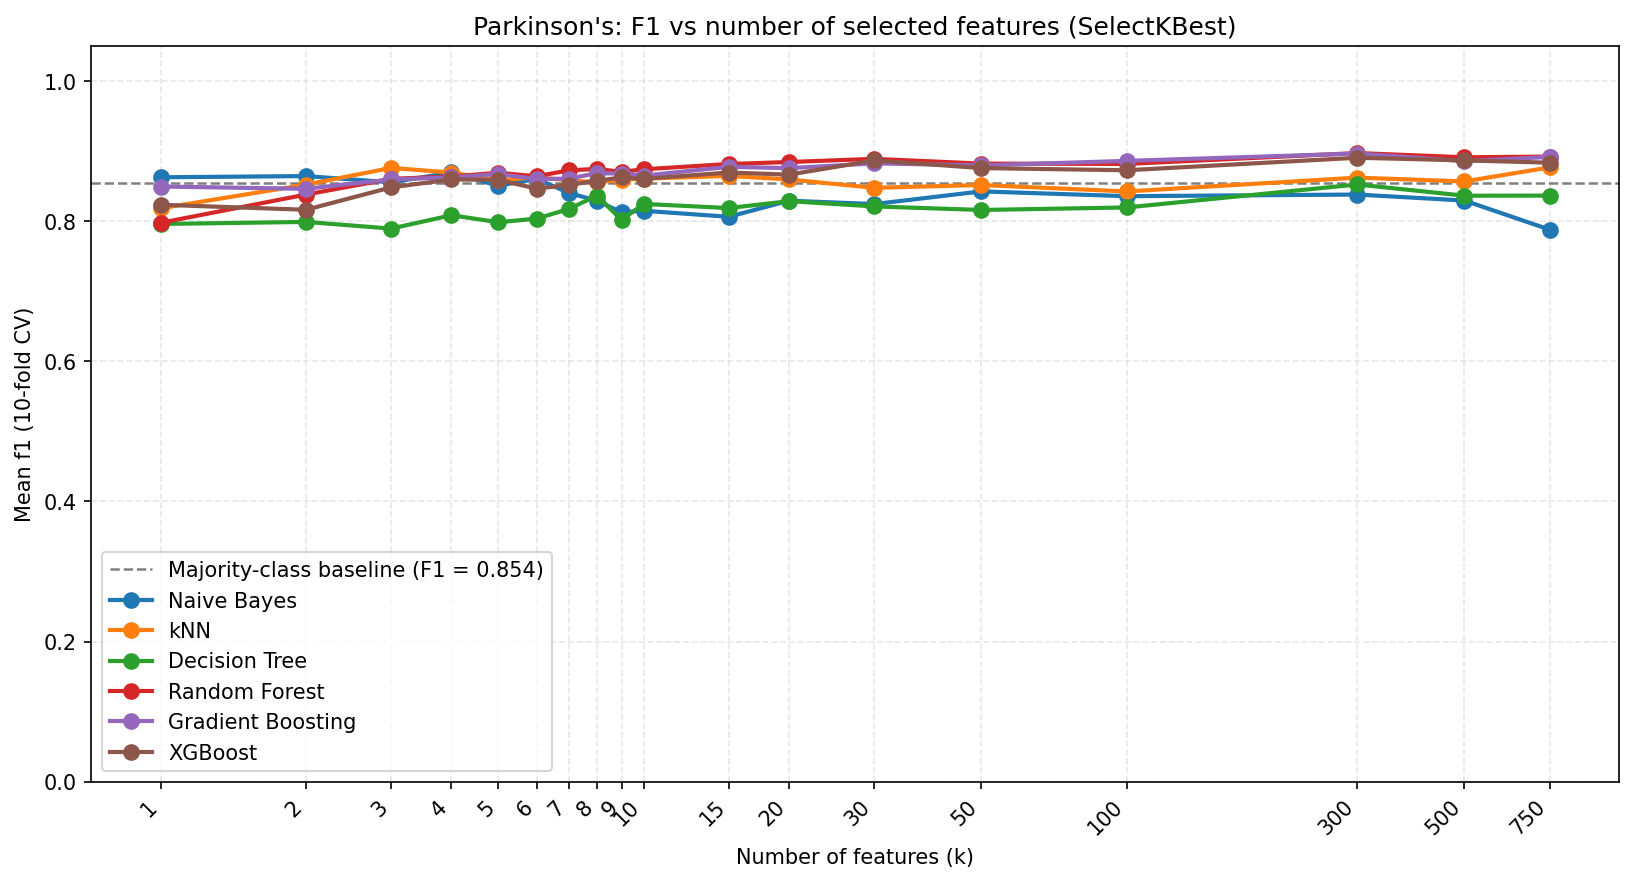
\includegraphics[width=0.95\textwidth]{feature_selection_sweep_f1.png}
    \caption{F1-score versus number of selected features for all six
    classifiers on Parkinson's. The dashed line marks the majority-class
    baseline of $F1 = 0.854$ --- the F1 a predictor that always outputs
    Parkinson's would achieve due to the 75/25 class imbalance.}
    \label{fig:pd_fs_f1}
\end{figure}

Figure~\ref{fig:pd_fs_f1} plots F1 as a function of the number of selected
features. The curves are nearly flat across the entire $k$ range: F1 varies by
less than 0.05 points between $k = 1$ and $k = 750$ for every classifier.
Several classifiers (Random Forest, Gradient Boosting, XGBoost) sit slightly
above the majority-class baseline of 0.854 across the full range. Decision
Tree and Naive Bayes fluctuate around it. Taken at face value, this would
suggest that feature selection has minimal effect.

However, this view is misleading because the F1 metric is dominated by the
class imbalance: a trivial predictor that always outputs Parkinson's would
already achieve $F1 = 0.854$. The fact that most classifiers are within 0.04
of this baseline at most values of $k$ indicates not that the classifiers are
skilled, but that the baseline itself is high. To see whether the classifiers
are actually learning, a metric immune to class imbalance is required.

\begin{figure}[H]
    \centering
    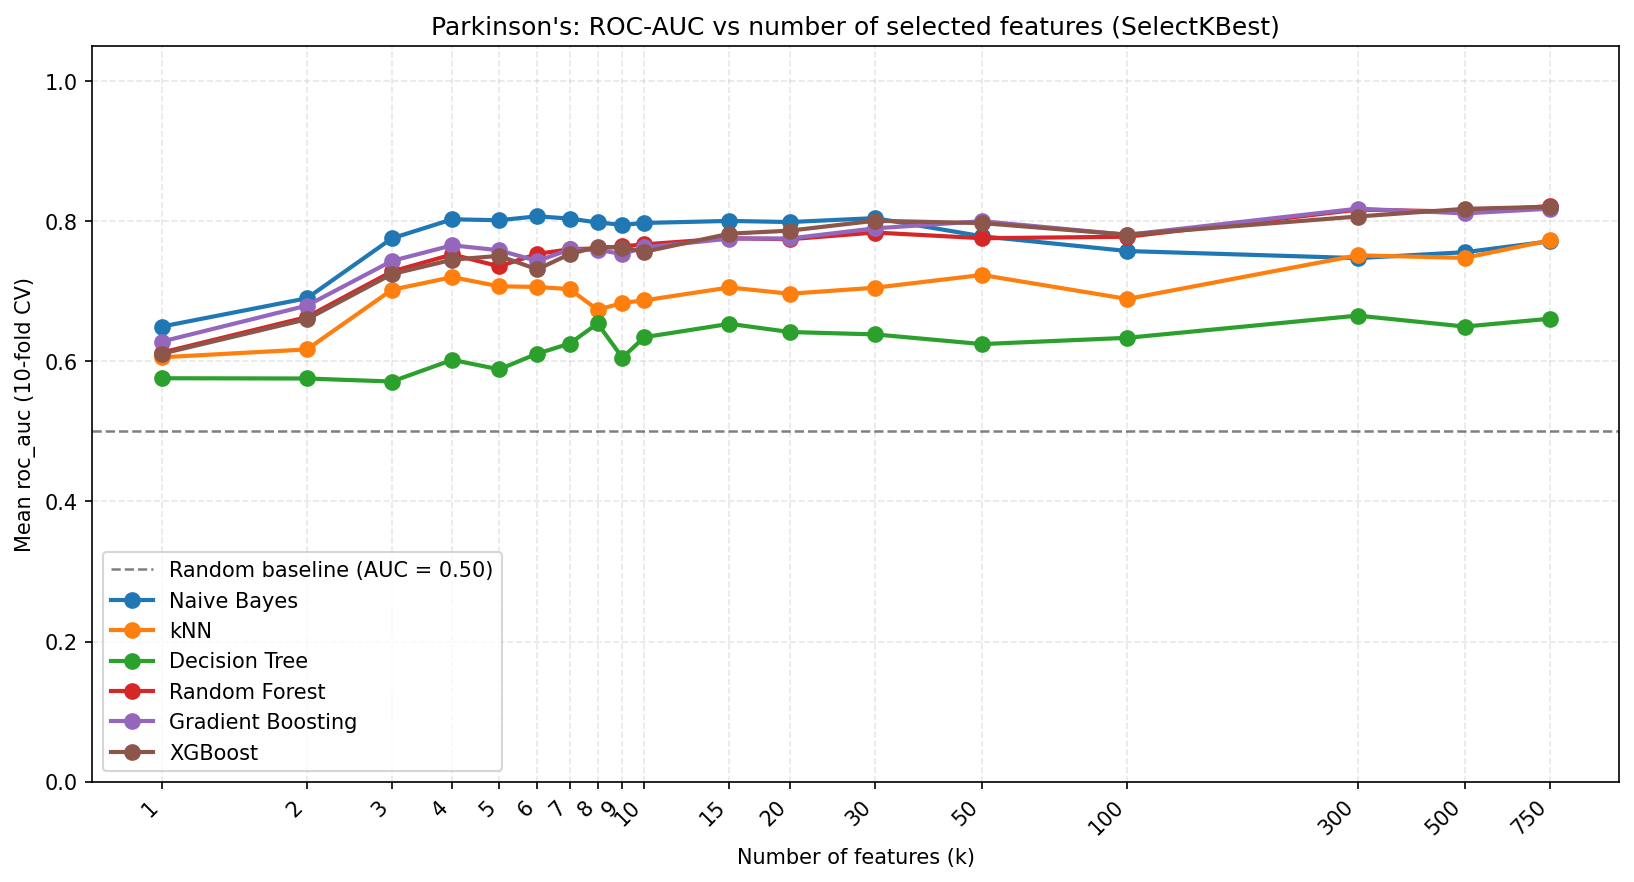
\includegraphics[width=0.95\textwidth]{feature_selection_sweep_roc_auc.png}
    \caption{ROC-AUC versus number of selected features. ROC-AUC is invariant
    to class imbalance --- a random classifier achieves 0.50 regardless of
    class proportions. The dashed line marks this random baseline.}
    \label{fig:pd_fs_roc}
\end{figure}

Figure~\ref{fig:pd_fs_roc} plots ROC-AUC against $k$. Unlike F1, ROC-AUC is
invariant to class imbalance: a random predictor scores 0.50 regardless of
class proportions. The curves now reveal clear structure. With a single
feature, all classifiers score between 0.58 and 0.65 --- modestly better than
random, but signalling weak discrimination. From $k = 1$ to $k = 10$, ensemble
methods rise steeply to approximately 0.78. Beyond $k = 15$ the curves
plateau, with marginal gains as $k$ grows further. Naive Bayes peaks early
(around $k = 5$ at ROC-AUC 0.80) and stays near that level. Decision Tree
alone fails to climb substantially, remaining around 0.60 ROC-AUC throughout,
consistent with its known sensitivity to high-dimensional noise.

This figure reveals that the signal in the Parkinson's dataset is concentrated
in the first ten or so features identified by ANOVA F-scores. Going beyond
$k = 15$ captures almost no additional discriminative information for most
classifiers.

\begin{figure}[H]
    \centering
    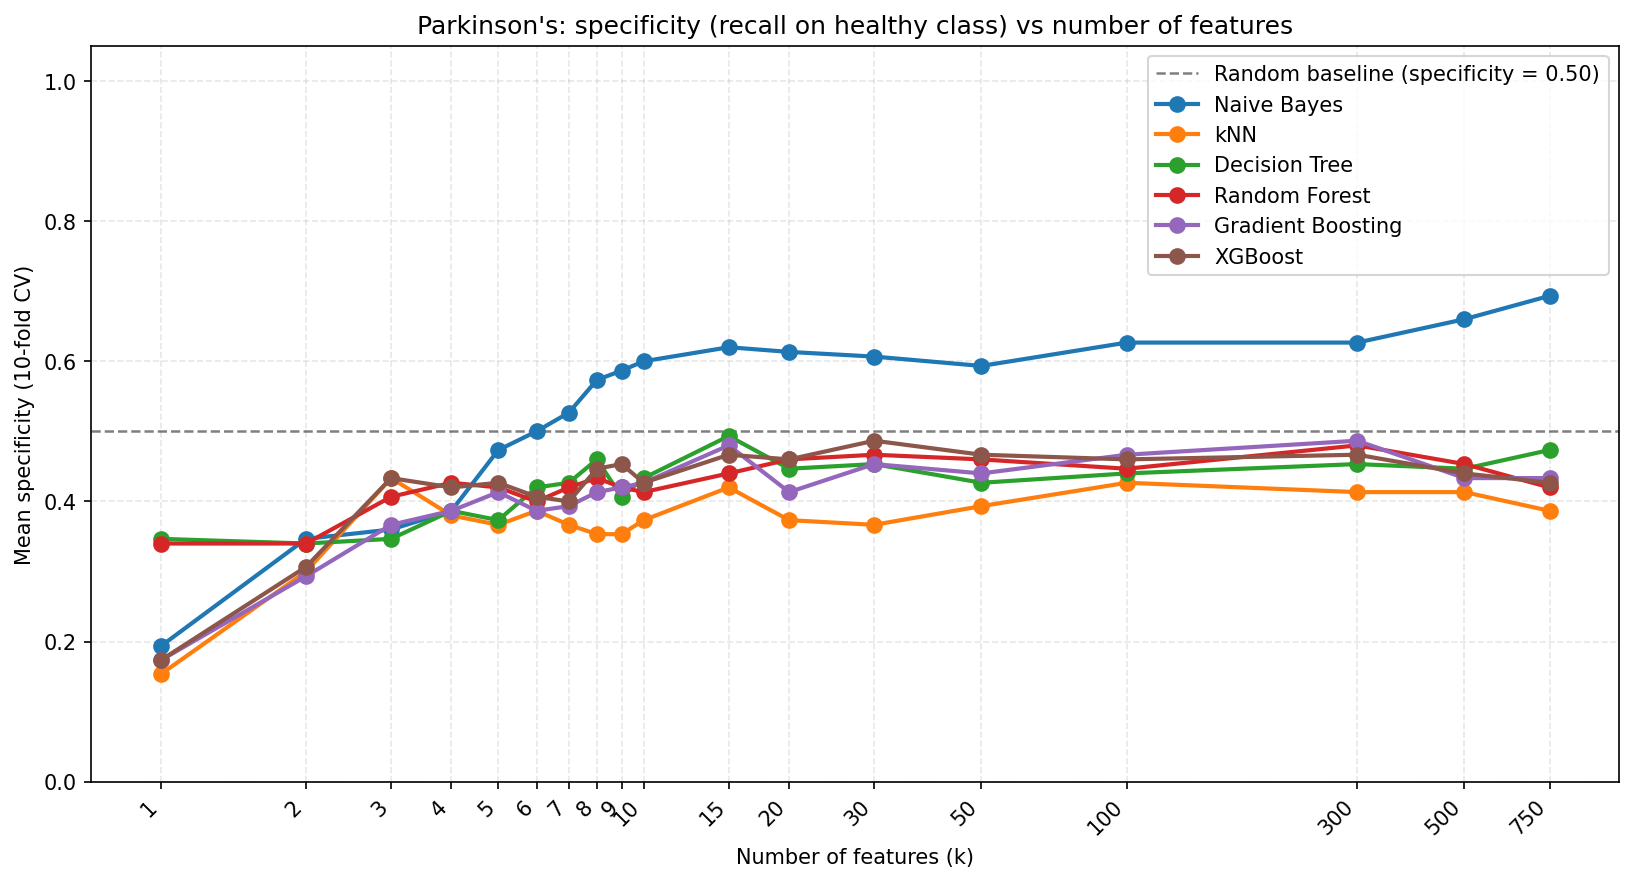
\includegraphics[width=0.95\textwidth]{feature_selection_sweep_specificity.png}
    \caption{Specificity (recall on the healthy control class) versus number
    of selected features. The dashed line marks the random baseline of 0.50.}
    \label{fig:pd_fs_specificity}
\end{figure}

Figure~\ref{fig:pd_fs_specificity} plots specificity --- the fraction of
actual healthy controls correctly identified as healthy. The pattern reveals
a systematic problem masked by the F1 view: only Naive Bayes consistently
exceeds the random-baseline specificity of 0.50 (reaching approximately 0.69
at $k = 750$). All tree-based ensembles plateau below 0.50, in the band
0.40--0.48, regardless of how many features are selected. This means that
across the full feature-count range, the ensemble classifiers misclassify
more than half of healthy controls as having Parkinson's. The high
sensitivity values that drive their high F1 scores are achieved by adopting a
strong bias toward predicting Parkinson's --- they catch nearly all positive
cases by predicting the positive class often.

Feature selection alone does not break this class-bias regime. Even at
$k = 750$, when all features are available, specificity for tree-based
ensembles remains in the 0.40--0.48 range. The bias is structural --- driven
by the 3:1 class imbalance in training data --- and cannot be addressed by
feature engineering.

\begin{figure}[H]
    \centering
    
\includegraphics[width=0.95\textwidth]{feature_selection_per_class_gradient_boosting.png}
    \caption{Per-class F1 for Gradient Boosting (the overall best Parkinson's
    classifier) as a function of the number of selected features. The two
    classes are shown as separate lines: Parkinson's recordings (orange) and
    healthy controls (blue).}
    \label{fig:pd_fs_perclass_gb}
\end{figure}

Figure~\ref{fig:pd_fs_perclass_gb} decomposes the Gradient Boosting
classifier's F1 by class. The Parkinson's-class F1 sits between 0.85 and 0.89
across the entire $k$ range --- high because the model correctly identifies
most actual Parkinson's recordings. The healthy-class F1 climbs more steeply
from 0.26 at $k = 1$ to approximately 0.55 by $k = 15$, then plateaus and
never exceeds 0.60. The persistent gap of approximately 0.30 F1 between the
two lines visualises the class-bias finding numerically: feature selection
narrows the gap somewhat at low $k$ but does not eliminate it.

\paragraph{Which features drive the signal?}

To understand why the discriminative signal saturates so quickly,
Table~\ref{tab:pd_top_features} lists the 20 most discriminative features
ranked by their ANOVA F-statistic on the training set. The pattern is
striking: 95\% of the top 20 features come from just two families --- MFCC
delta coefficients, which measure how the spectral envelope of speech changes
between consecutive frames, and TQWT (Tunable-Q Wavelet Transform)
decomposition statistics, which capture multi-resolution time-frequency
properties at specific decomposition levels. Beyond $k \approx 15$,
additional features are predominantly correlated variants of measurements
that the top-ranked features already capture --- different MFCC coefficients
of the same speech segments, or TQWT statistics at neighbouring decomposition
levels. This concentration explains the ROC-AUC plateau quantitatively.

\begin{table}[H]
    \centering
    \caption{The 20 most discriminative individual features in the
    Parkinson's training set, ranked by ANOVA F-statistic.}
    \label{tab:pd_top_features}
    \begin{tabular}{rllr}
        \toprule
        Rank & Feature & Family & F-score \\
        \midrule
         1 & \texttt{mean\_MFCC\_2nd\_coef}           & MFCC cepstral & 118.1 \\
         2 & \texttt{tqwt\_kurtosisValue\_dec\_27}    & TQWT          & 112.8 \\
         3 & \texttt{tqwt\_kurtosisValue\_dec\_26}    & TQWT          &  99.5 \\
         4 & \texttt{std\_9th\_delta\_delta}          & MFCC delta    &  99.4 \\
         5 & \texttt{std\_8th\_delta\_delta}          & MFCC delta    &  98.3 \\
         6 & \texttt{std\_7th\_delta\_delta}          & MFCC delta    &  93.1 \\
         7 & \texttt{std\_6th\_delta\_delta}          & MFCC delta    &  92.0 \\
         8 & \texttt{tqwt\_stdValue\_dec\_12}         & TQWT          &  87.7 \\
         9 & \texttt{std\_8th\_delta}                 & MFCC delta    &  86.8 \\
        10 & \texttt{std\_9th\_delta}                 & MFCC delta    &  85.5 \\
        11 & \texttt{tqwt\_minValue\_dec\_12}         & TQWT          &  84.8 \\
        12 & \texttt{tqwt\_maxValue\_dec\_12}         & TQWT          &  82.2 \\
        13 & \texttt{std\_6th\_delta}                 & MFCC delta    &  81.0 \\
        14 & \texttt{tqwt\_entropy\_log\_dec\_12}     & TQWT          &  77.4 \\
        15 & \texttt{tqwt\_stdValue\_dec\_11}         & TQWT          &  77.4 \\
        16 & \texttt{std\_11th\_delta\_delta}         & MFCC delta    &  77.2 \\
        17 & \texttt{std\_7th\_delta}                 & MFCC delta    &  76.0 \\
        18 & \texttt{tqwt\_entropy\_shannon\_dec\_16} & TQWT          &  74.7 \\
        19 & \texttt{std\_10th\_delta\_delta}         & MFCC delta    &  73.5 \\
        20 & \texttt{tqwt\_entropy\_shannon\_dec\_15} & TQWT          &  73.0 \\
        \bottomrule
    \end{tabular}
\end{table}

Three findings summarise the feature-selection analysis for Parkinson's.
First, the discriminative signal is concentrated in approximately the first
ten features ranked by ANOVA F-statistic: ROC-AUC plateaus by $k = 15$ for
ensemble methods, a plateau the top-features table above explains
mechanistically. Second, the F1 metric is misleading in this setting because
of class imbalance --- a trivial baseline already scores 0.854, leaving
little headroom for visible classifier improvement. Third, feature selection
does not address the underlying class-bias problem --- most classifiers
continue to misidentify healthy controls regardless of $k$.

% ---------------------------------------------------------------------
\subsubsection{PCA Analysis}
% ---------------------------------------------------------------------

Principal Component Analysis was investigated as an alternative dimensionality
reduction approach. The number of principal components was swept across eight
values from 5 to 500, with all six classifiers evaluated at each value using
ten-fold patient-grouped cross-validation.

\begin{table}[H]
    \centering
    \caption{PCA at 95\% variance (approximately 158 components) versus the
    scaled baseline.}
    \label{tab:pd_pca}
    \begin{tabular}{lrrr}
        \toprule
        Model              & Scaled F1 & Scaled + PCA F1 & Difference \\
        \midrule
        Naive Bayes        & 0.7913 & 0.8271 & $+0.0358$ \\
        kNN                & 0.8774 & 0.8786 & $+0.0012$ \\
        Decision Tree      & 0.8202 & 0.8098 & $-0.0104$ \\
        Random Forest      & 0.8868 & 0.8641 & $-0.0227$ \\
        Gradient Boosting  & 0.8895 & 0.8770 & $-0.0125$ \\
        XGBoost            & 0.8803 & 0.8903 & $+0.0100$ \\
        \bottomrule
    \end{tabular}
\end{table}

\begin{figure}[H]
    \centering
    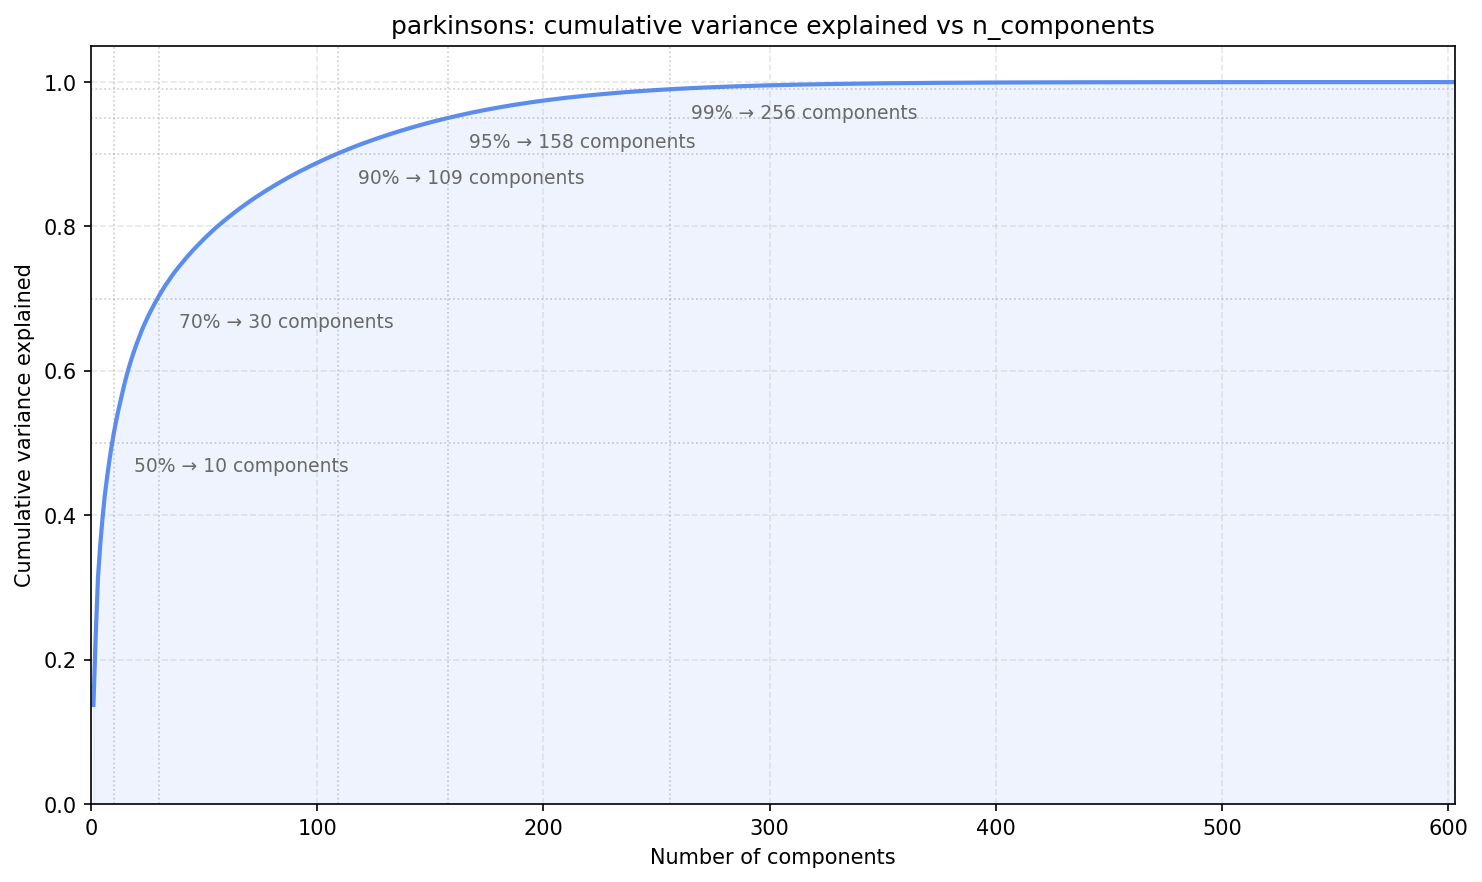
\includegraphics[width=0.95\textwidth]{pca_variance_explained.png}
    \caption{Cumulative variance explained as a function of the number of
    principal components for the Parkinson's training data. The plot
    annotates the number of components needed to reach 50\%, 70\%, 90\%,
    95\%, and 99\% of total variance.}
    \label{fig:pd_pca_variance}
\end{figure}

Figure~\ref{fig:pd_pca_variance} confirms that the Parkinson's dataset is
highly redundant: 50\% of total variance is captured in just 10 components,
90\% in 109 components, and 99\% in 256 components. This is consistent with
the structure of the voice-acoustic features: many measurements (jitter
variants, shimmer variants, MFCC coefficients at different frames) derive
from the same underlying signal and are therefore highly correlated.

\begin{figure}[H]
    \centering
    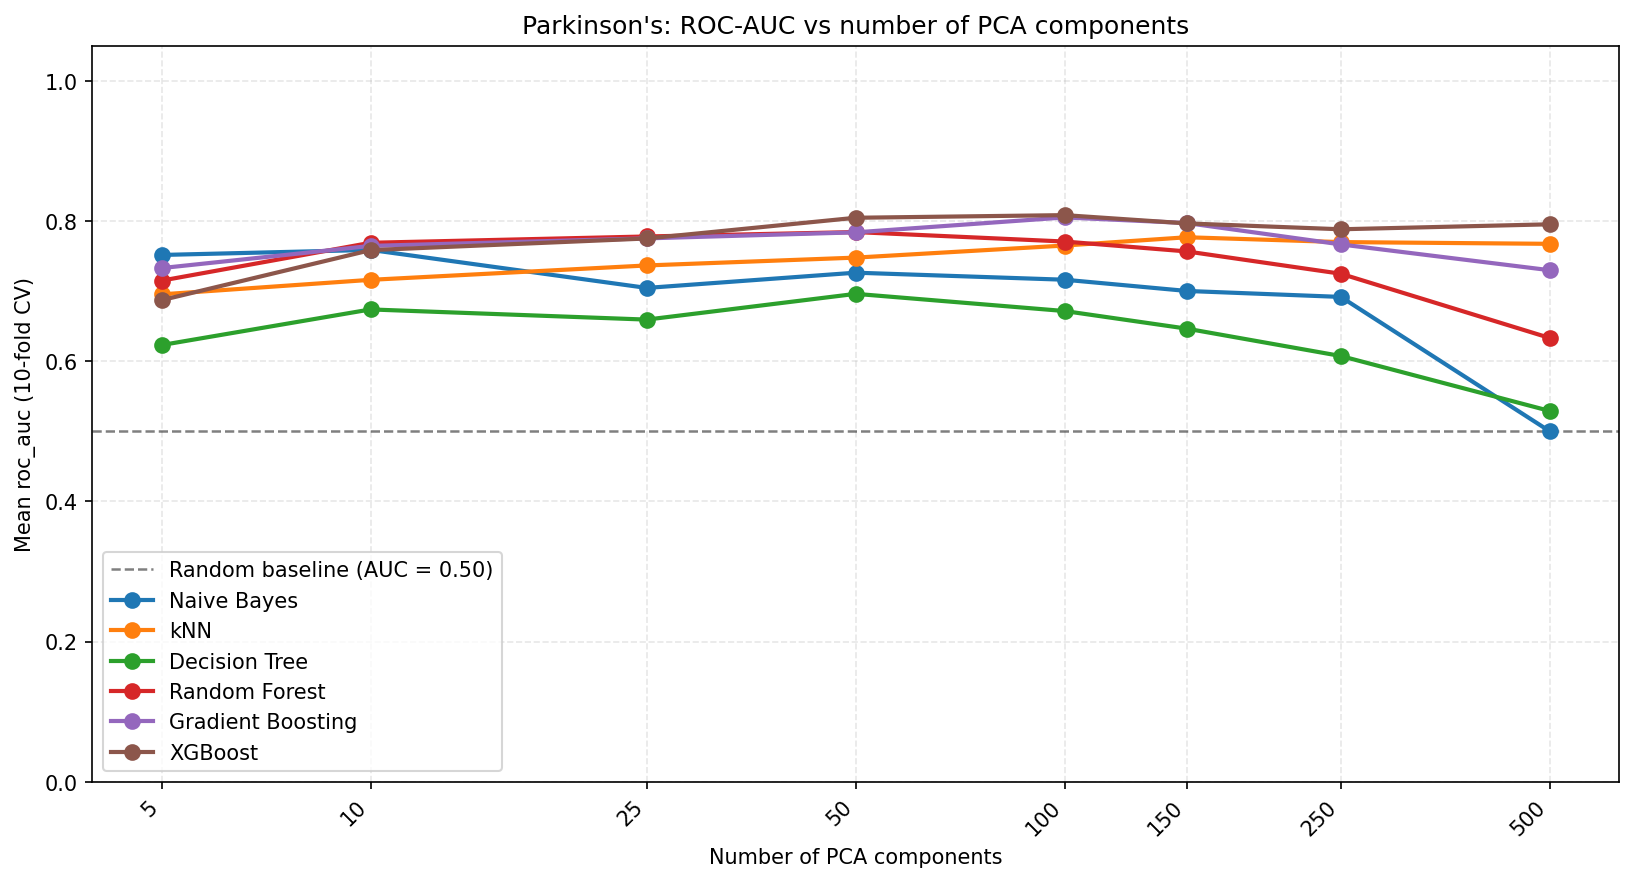
\includegraphics[width=0.95\textwidth]{pca_sweep_roc_auc.png}
    \caption{ROC-AUC versus number of PCA components, for all six classifiers
    on Parkinson's. The dashed line marks the random-baseline ROC-AUC of
    0.50.}
    \label{fig:pd_pca_roc}
\end{figure}

Figure~\ref{fig:pd_pca_roc} reveals a striking failure mode at the high end
of the component range. From 5 to approximately 250 components, ROC-AUC for
all classifiers stays in the 0.70--0.80 band. At 500 components --- beyond
the 256-component threshold where 99\% of variance is captured --- the
remaining ``components'' are essentially noise. Naive Bayes collapses to
ROC-AUC of 0.50 (literally random discrimination), Decision Tree falls to
0.53, and Random Forest drops from 0.78 to 0.63. kNN and XGBoost remain
relatively stable.

This is a cautionary finding: PCA is not a free transformation, and applying
it with too many components is actively harmful for several model families,
particularly methods that assume feature independence (Naive Bayes) or that
overfit to weak signals (single-tree models). A sensible operating range is
50--150 components, corresponding to approximately 80--92\% of variance
retained.

\paragraph{What do the top principal components represent?}

The feature-ranking analysis of Table~\ref{tab:pd_top_features} ordered
individual features by their univariate class-separation power (an ANOVA
F-statistic) and showed that MFCC delta and TQWT features carry the strongest
discriminative signal. PCA orders \emph{directions} by variance, which is a
different criterion. Table~\ref{tab:pd_pc_loadings} reports, for each of the
first ten principal components, the single feature with the largest absolute
loading on that component and the feature family that dominates its top-10
loadings. The pattern is informative: the first six PCs --- accounting for
roughly 43\% of total variance --- are entirely Wavelet- and TQWT-dominated;
MFCC delta does not become a major contributor to any component until PC7,
by which point still only 45\% of variance has been captured. The largest
modes of variation in the scaled feature space describe wavelet- and
TQWT-domain structure shared across recordings, while the MFCC delta
features that drive the strongest univariate separation contribute
comparatively little to overall variance. This mismatch between
``variance-dominant'' and ``discrimination-dominant'' directions helps
explain why PCA only meaningfully improves Naive Bayes in
Table~\ref{tab:pd_pca}: projecting onto top components preserves variance
but does not preferentially preserve the directions that separate classes.

\begin{table}[H]
    \centering
    \caption{Top contributing feature and dominant feature family of the
    first ten principal components of the (scaled) Parkinson's training
    set. The dominant family is the most frequent family among the ten
    features with the largest absolute loading on each component.}
    \label{tab:pd_pc_loadings}
    \begin{tabular}{rrll}
        \toprule
        PC & Var.\ (\%) & Top feature (largest $|$loading$|$) & Dominant family (top-10) \\
        \midrule
        1  & 13.73 & \texttt{app\_LT\_entropy\_shannon\_5\_coef} & Wavelet     \\
        2  & 9.56  & \texttt{tqwt\_maxValue\_dec\_8}             & TQWT        \\
        3  & 8.02  & \texttt{det\_entropy\_log\_2\_coef}         & Wavelet     \\
        4  & 4.56  & \texttt{tqwt\_minValue\_dec\_31}            & TQWT        \\
        5  & 3.66  & \texttt{tqwt\_entropy\_shannon\_dec\_5}     & TQWT        \\
        6  & 3.17  & \texttt{tqwt\_maxValue\_dec\_21}            & TQWT        \\
        7  & 2.48  & \texttt{tqwt\_energy\_dec\_6}               & MFCC delta  \\
        8  & 2.29  & \texttt{tqwt\_stdValue\_dec\_28}            & TQWT        \\
        9  & 2.07  & \texttt{det\_LT\_entropy\_shannon\_5\_coef} & TQWT        \\
        10 & 1.82  & \texttt{tqwt\_kurtosisValue\_dec\_4}        & TQWT        \\
        \bottomrule
    \end{tabular}
\end{table}

% ---------------------------------------------------------------------
\subsubsection{Hyperparameter Sweep Analysis}\label{sec:pd_sweeps}
% ---------------------------------------------------------------------

For each tunable classifier (kNN, Decision Tree, Random Forest, Gradient
Boosting, and XGBoost) the two principal hyperparameters were swept using
10-fold patient-grouped CV, with the secondary hyperparameter shown as
separate lines on each plot and the remaining hyperparameters held at their
defaults. Each classifier was evaluated on its Stage-1 best preprocessing
configuration. Naive Bayes is omitted: the variant used (Gaussian Naive
Bayes) has no tunable hyperparameters in the search space considered. For
every sweep cell, all six metrics --- accuracy, precision, recall,
specificity, F1, and ROC-AUC --- are recorded; reporting them side-by-side
rather than F1 alone is important here because, as the following plots show,
the choice of metric noticeably changes which configuration appears optimal.

\paragraph{k-Nearest Neighbors.}

Figure~\ref{fig:pd_sweep_knn} sweeps the number of neighbors $k$ across
30 values from 1 to 150, with one line per distance metric. The distance
metric is not just a tuning detail: Manhattan distance peaks at very small
$k$ ($k=3$) and degrades steadily as $k$ grows, while Chebyshev distance
behaves in the opposite direction, peaking around $k = 35\text{--}80$.
Euclidean sits in between. Specificity collapses toward zero at small $k$
for all three metrics --- a sign that the closest neighbors are
overwhelmingly PD patients in this 75/25-imbalanced dataset. Best F1:
$k = 35$, Chebyshev, F1 $= 0.886$.

\begin{figure}[H]
    \centering
    
\includegraphics[width=\textwidth]{classifier_sweep_knn.png}
    \caption{kNN hyperparameter sweep on Parkinson's: F1 and five other
    metrics versus the number of neighbors, segmented by distance metric.}
    \label{fig:pd_sweep_knn}
\end{figure}

\paragraph{Decision Tree.}

Figure~\ref{fig:pd_sweep_dt} is a textbook overfitting curve. F1 and
accuracy both peak at \texttt{max\_depth} $= 2$ and drop monotonically as
depth grows. The trade-off across metrics is striking: deeper trees lose
F1 but \emph{gain} precision and specificity --- the deeper model becomes
more selective, predicting PD less often. With only $\sim 200$ training
samples and 753 features, the tree exhausts its splitting budget before
depth $\approx 25$ and the curves flatten. Best F1: \texttt{max\_depth} $= 2$,
\texttt{min\_samples\_leaf} $= 0.001$, F1 $= 0.864$.

\begin{figure}[H]
    \centering
    
\includegraphics[width=\textwidth]{classifier_sweep_decision_tree.png}
    \caption{Decision Tree hyperparameter sweep on Parkinson's: ten
    \texttt{max\_depth} values, four \texttt{min\_samples\_leaf} values,
    all six metrics.}
    \label{fig:pd_sweep_dt}
\end{figure}

\paragraph{Random Forest.}

Figure~\ref{fig:pd_sweep_rf} shows F1 rising rapidly from 5 to about 100
trees and then saturating around F1 $\approx 0.89$. The
\texttt{max\_depth} lines for $25$ and $70$ are exactly superimposed --- a
direct observation that the individual trees stop splitting well before
depth $25$ (the dataset's pure-leaf criterion bites first), so any depth
limit above $\sim 25$ is non-binding. ROC-AUC tracks F1 closely on this
classifier, and specificity is the noisiest metric. Best F1:
$100$ trees, \texttt{max\_depth} $= 25$, F1 $= 0.895$.

\begin{figure}[H]
    \centering
    
\includegraphics[width=\textwidth]{classifier_sweep_random_forest.png}
    \caption{Random Forest hyperparameter sweep on Parkinson's: fourteen
    \texttt{n\_estimators} values, three \texttt{max\_depth} values.}
    \label{fig:pd_sweep_rf}
\end{figure}

\paragraph{Gradient Boosting.}

Figure~\ref{fig:pd_sweep_gb} is the most informative panel for the
multi-metric framing. F1 peaks at \texttt{n\_estimators} $= 50$ with
\texttt{max\_depth} $= 5$ and then \emph{declines slightly}, but ROC-AUC
continues to climb past $n = 50$, peaking at $n = 250$. The argmax under F1
and under ROC-AUC therefore disagree on this classifier --- the F1-optimal
model has ROC-AUC $= 0.822$, whereas the ROC-AUC-optimal model is more
extensively boosted ($n = 250$) and trades a fraction of F1 for $+0.017$
ROC-AUC. Specificity climbs from $0.05$ at $n = 5$ to $\sim 0.47$ at
$n \geq 50$, the largest specificity range observed in any sweep. Shallow
trees (\texttt{max\_depth} $= 5$) dominate deeper ones across every metric.
Best F1: $n = 50$, \texttt{max\_depth} $= 5$, F1 $= 0.900$ --- the highest F1
recorded on Parkinson's.

\begin{figure}[H]
    \centering
    
\includegraphics[width=\textwidth]{classifier_sweep_gradient_boosting.png}
    \caption{Gradient Boosting hyperparameter sweep on Parkinson's: ten
    \texttt{n\_estimators} values, three \texttt{max\_depth} values.}
    \label{fig:pd_sweep_gb}
\end{figure}

\paragraph{XGBoost.}

Figure~\ref{fig:pd_sweep_xgb} has the smallest variation of any sweep
(F1 spans only $0.873\text{--}0.891$, a range of $0.018$). The
\texttt{max\_depth} lines for $10$, $25$, and $50$ are all coincident
--- the same depth-saturation effect that appears in Random Forest. Only
\texttt{max\_depth} $= 5$ traces a distinct curve, peaking at
\texttt{n\_estimators} $= 75$ with F1 $= 0.891$. The model is essentially
insensitive to further tuning beyond the depth choice.

\begin{figure}[H]
    \centering
    
\includegraphics[width=\textwidth]{classifier_sweep_xgboost.png}
    \caption{XGBoost hyperparameter sweep on Parkinson's: ten
    \texttt{n\_estimators} values, four \texttt{max\_depth} values.}
    \label{fig:pd_sweep_xgb}
\end{figure}

\paragraph{Cross-classifier synthesis.}

Ranking the five tunable classifiers by their best CV-F1: Gradient Boosting
($0.900$), Random Forest ($0.895$), XGBoost ($0.891$), kNN ($0.886$),
Decision Tree ($0.864$). The four ensemble or instance-based methods cluster
within $0.014$ of each other --- on this dataset, the choice of model family
matters less than the choice of preprocessing (cf.\
Tables~\ref{tab:pd_scaling}, \ref{tab:pd_feature_selection},
\ref{tab:pd_pca}) and less than the choice of primary metric. Two recurring
observations across the sweeps are worth flagging. First, the F1-optimal
configuration is not always the ROC-AUC-optimal one (most visibly in
Gradient Boosting and kNN): committing to a single primary metric quietly
fixes a methodological choice. Second, the tree-based ensembles saturate
their depth budget before reaching the larger \texttt{max\_depth} limits on
the sweep, so the deeper-line variants overlap exactly --- a property of the
dataset's geometry (high feature count, low sample count) rather than of
the algorithms themselves.

% ---------------------------------------------------------------------
\subsubsection{Final Parkinson's Model}\label{sec:pd_final}
% ---------------------------------------------------------------------

Stage 2 ran a per-classifier \texttt{GridSearchCV} on each model's
Stage-1-best preprocessing using the reduced grids in
\texttt{configs/hyperparameters.yaml}. Table~\ref{tab:pd_tuning} summarises
the tuned CV-F1 for each classifier. Gradient Boosting wins overall, edging
Random Forest by $0.005$ and XGBoost by $0.012$. The full chosen
configuration is Gradient Boosting on \emph{scaled} features with
\texttt{learning\_rate}~$=0.1$, \texttt{max\_depth}~$=5$,
\texttt{n\_estimators}~$=50$, \texttt{max\_features}~$=\sqrt{n}$.

\begin{table}[H]
    \centering
    \caption{Per-classifier tuned CV-F1 from Stage 2 grid search on
    Parkinson's. The chosen preprocessing is the Stage-1 winner from
    Table~\ref{tab:pd_overall}.}
    \label{tab:pd_tuning}
    \begin{tabular}{lll>{\centering\arraybackslash}p{2.3cm}}
        \toprule
        Classifier & Preprocessing & Tuned CV-F1 & Rank \\
        \midrule
        Naive Bayes       & scaled + feature selection & $0.8424$ & 6 \\
        kNN               & scaled + PCA               & $0.8859$ & 4 \\
        Decision Tree     & raw                        & $0.8439$ & 5 \\
        Random Forest     & raw                        & $0.8949$ & 2 \\
        \textbf{Gradient Boosting} & \textbf{scaled}   & $\mathbf{0.8997}$ & \textbf{1} \\
        XGBoost           & scaled + PCA               & $0.8880$ & 3 \\
        \bottomrule
    \end{tabular}
\end{table}

\paragraph{Held-out test evaluation.}

Refitting the tuned Gradient Boosting on the full training set and
evaluating on the 20\% held-out test split ($n = 153$, of which 111 PD and
42 Healthy) produced the aggregate metrics in Table~\ref{tab:pd_final}.
The headline F1 of $0.905$ is $+0.051$ above the majority-class baseline of
$0.854$ established in \S\ref{sec:baselines}, and ROC-AUC of $0.938$
indicates substantially better class separability than the F1 alone
suggests --- a recurring observation throughout this analysis.

\begin{table}[H]
    \centering
    \caption{Test-set metrics for the tuned Gradient Boosting model on
    Parkinson's. The \emph{Healthy} and \emph{PD} columns are the per-class
    decomposition; \emph{Aggregate} is the binary (positive-class) view that
    F1, precision, and recall report by default.}
    \label{tab:pd_final}
    \begin{tabular}{lrrr}
        \toprule
        Metric & Aggregate & Healthy & PD \\
        \midrule
        Precision & $0.833$ & $0.952$ & $0.833$ \\
        Recall    & $0.991$ & $0.476$ & $0.991$ \\
        F1        & $0.905$ & $0.635$ & $0.905$ \\
        Support   & $153$   & $42$    & $111$   \\
        \midrule
        Accuracy  & \multicolumn{3}{c}{$0.850$} \\
        ROC-AUC   & \multicolumn{3}{c}{$0.938$} \\
        \bottomrule
    \end{tabular}
\end{table}

\begin{figure}[H]
    \centering
    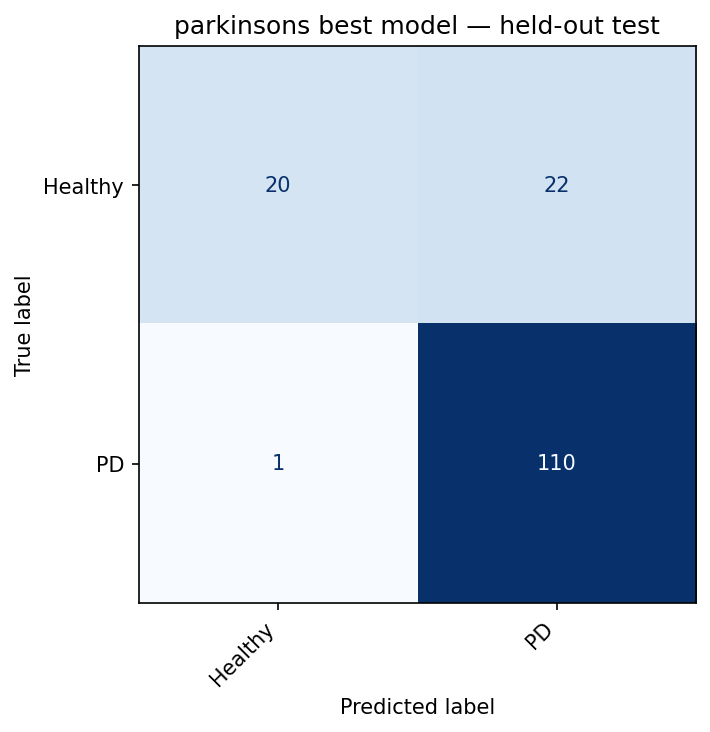
\includegraphics[width=0.55\textwidth]{../artifacts/final/parkinsons/confusion_matrix.png}
    \caption{Confusion matrix for the tuned Gradient Boosting model on the
    held-out Parkinson's test set. Rows are true labels, columns are
    predictions.}
    \label{fig:pd_confusion}
\end{figure}

The confusion matrix in Figure~\ref{fig:pd_confusion} exposes the per-class
asymmetry that the aggregate F1 hides. Of $111$ PD test patients, the model
correctly identifies $110$ (recall $= 0.991$); only one PD case is missed.
Of $42$ Healthy test patients, however, the model correctly identifies only
$20$ (specificity $= 0.476$): more than half of the healthy patients are
predicted as PD. Per-class F1 reflects this: PD F1 $= 0.905$ versus Healthy
F1 $= 0.635$.

This pattern is not unique to the chosen model. Section~\ref{sec:pd_sweeps}
showed recall sitting at $0.95\text{--}1.00$ across nearly every cell of
every classifier's hyperparameter sweep while specificity swung between $0$
and $0.47$. The 75/25 class distribution biases all six classifier families
toward predicting PD aggressively, and threshold tuning rather than further
hyperparameter search would be the next lever for trading PD recall against
Healthy specificity. The ROC-AUC of $0.938$ confirms that this trade-off
exists in the model's score distribution: there is real separability
available; the default decision threshold simply sits closer to the
high-recall end of the operating curve than the symmetric point.

% =====================================================================
\subsection{Covertype Results}
% =====================================================================

This section mirrors the Parkinson's results, but with Covertype-specific
metrics. Since Covertype is a multiclass classification problem, accuracy is
reported together with macro-averaged metrics and per-class results.

% ---------------------------------------------------------------------
\subsubsection{Overall Model Comparison}
% ---------------------------------------------------------------------

\begin{table}[H]
    \centering
    \caption{Overall comparison of the six classifiers on Covertype, each
    evaluated with its Stage-2 best preprocessing and tuned hyperparameters.
    Metrics are 10-fold cross-validation means on the training set.}
    \label{tab:ct_overall}
    \begin{tabular}{llrrrr}
        \toprule
        Model & Best preprocessing & Accuracy & Macro F1 & Macro Precision & Macro Recall \\
        \midrule
        Naive Bayes        & raw                  & $0.5996$ & $0.5528$ & $0.6526$ & $0.5996$ \\
        kNN                & raw                  & $0.7943$ & $0.7885$ & $0.7885$ & $0.7943$ \\
        Decision Tree      & raw                  & $0.7380$ & $0.7365$ & $0.7374$ & $0.7380$ \\
        Random Forest      & scaled + FS          & $0.8271$ & $0.8240$ & $0.8248$ & $0.8271$ \\
        Gradient Boosting  & raw                  & $0.8304$ & $0.8285$ & $0.8290$ & $0.8304$ \\
        XGBoost            & raw                  & $0.8305$ & $0.8281$ & $0.8287$ & $0.8305$ \\
        \bottomrule
    \end{tabular}
\end{table}

The three tree-based ensembles cluster within $0.003$ macro F1 of each other
(Random Forest $0.824$, XGBoost $0.828$, Gradient Boosting $0.829$): on
this dataset the choice among them is essentially a coin flip, and the
selection of Gradient Boosting in \S\ref{sec:ct_final} reflects a CV margin
that is much smaller than a single standard deviation. kNN at $k = 1$
follows at macro F1 $= 0.789$, Decision Tree at $0.737$, and Gaussian
Naive Bayes at $0.553$ --- well above the balanced-class random baseline of
$1/7 \approx 0.143$ but the only model that fails to cross macro F1 $= 0.7$.
A signature of the balanced subsampling carried out in
\S\ref{sec:covertype} is visible in the table: accuracy equals macro recall
to four decimal places for every classifier (because micro and macro recall
coincide when every class has equal support), so on this dataset the two
columns carry the same information.

% ---------------------------------------------------------------------
\subsubsection{Effect of Scaling}
% ---------------------------------------------------------------------

\begin{table}[H]
    \centering
    \caption{Effect of scaling on Covertype: cross-validation mean macro F1
    for each classifier under raw and scaled features.}
    \label{tab:ct_scaling}
    \begin{tabular}{lrrr}
        \toprule
        Model              & Raw Macro F1 & Scaled Macro F1 & Difference \\
        \midrule
        Naive Bayes        & 0.5528 & 0.3748 & $-0.1779$ \\
        kNN                & 0.7396 & 0.7280 & $-0.0117$ \\
        Decision Tree      & 0.7344 & 0.7339 & $-0.0005$ \\
        Random Forest      & 0.8173 & 0.8175 & $+0.0003$ \\
        Gradient Boosting  & 0.7750 & 0.7749 & $-0.0002$ \\
        XGBoost            & 0.8247 & 0.8247 & $+0.0000$ \\
        \bottomrule
    \end{tabular}
\end{table}

\begin{figure}[H]
    \centering
    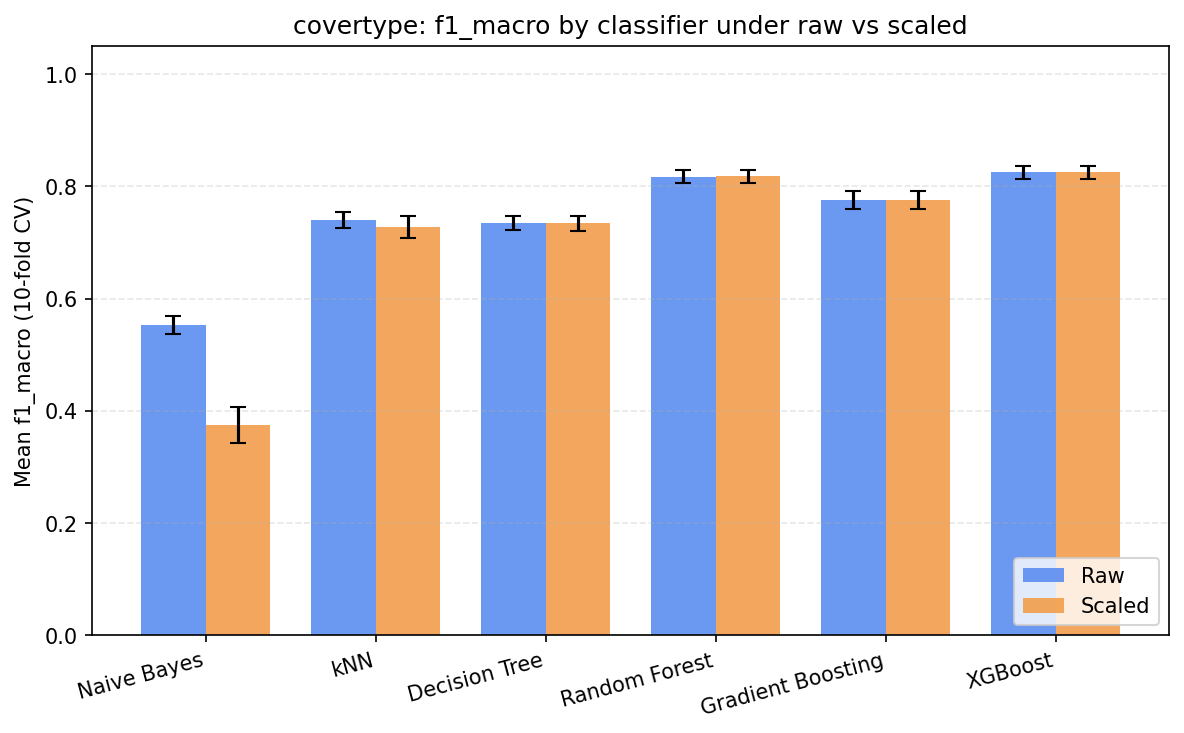
\includegraphics[width=0.9\textwidth]{../artifacts/final/covertype/plots/scaling_impact.png}
    \caption{Macro F1-score for each classifier on Covertype under raw versus
    scaled preprocessing.}
    \label{fig:ct_scaling}
\end{figure}

Scaling produces the largest single negative effect observed in either
dataset's preprocessing analysis: Naive Bayes loses nearly eighteen macro F1
points (0.553 $\to$ 0.375) under standard scaling. This is consistent with
the Covertype mixed feature structure --- ten continuous physical
measurements (elevation, slope, distances) and forty-four one-hot binary
indicators (wilderness area, soil type). Rescaling the continuous columns to
mean zero, unit variance creates a representational mismatch with the
unrescaled $0/1$ binary columns; Gaussian Naive Bayes's per-feature Gaussian
assumption then no longer applies coherently across the feature space,
distorting the posterior computation.

The remaining five classifiers are essentially unaffected by scaling
(differences within $\pm 0.012$ macro F1), and four of them register zero
change to four decimal places. For Covertype, the conclusion of the
scaling experiment is therefore simple: scaling provides no benefit to any
classifier and substantially damages Naive Bayes, so the raw-features
configuration is the safer default. The mechanism underlying the kNN result
specifically --- why a preprocessing step that yielded a large gain on
Parkinson's produces no effect here --- is examined in the cross-dataset
discussion of \S\ref{sec:comparison}, where the feature-level breakdowns in
\S\ref{sec:pd_features} and \S\ref{sec:ct_features} are available.

% ---------------------------------------------------------------------
\subsubsection{Feature Selection Analysis}\label{sec:ct_features}
% ---------------------------------------------------------------------

\begin{table}[H]
    \centering
    \caption{Feature selection at $k = 30$ (of 54 available features) versus
    the scaled baseline.}
    \label{tab:ct_feature_selection}
    \begin{tabular}{lrrr}
        \toprule
        Model              & Scaled Macro F1 & Scaled + FS Macro F1 & Difference \\
        \midrule
        Naive Bayes        & 0.3748 & 0.3944 & $+0.0195$ \\
        kNN                & 0.7280 & 0.7339 & $+0.0060$ \\
        Decision Tree      & 0.7339 & 0.7327 & $-0.0012$ \\
        Random Forest      & 0.8175 & 0.8202 & $+0.0027$ \\
        Gradient Boosting  & 0.7749 & 0.7720 & $-0.0029$ \\
        XGBoost            & 0.8247 & 0.8208 & $-0.0039$ \\
        \bottomrule
    \end{tabular}
\end{table}

\begin{figure}[H]
    \centering
    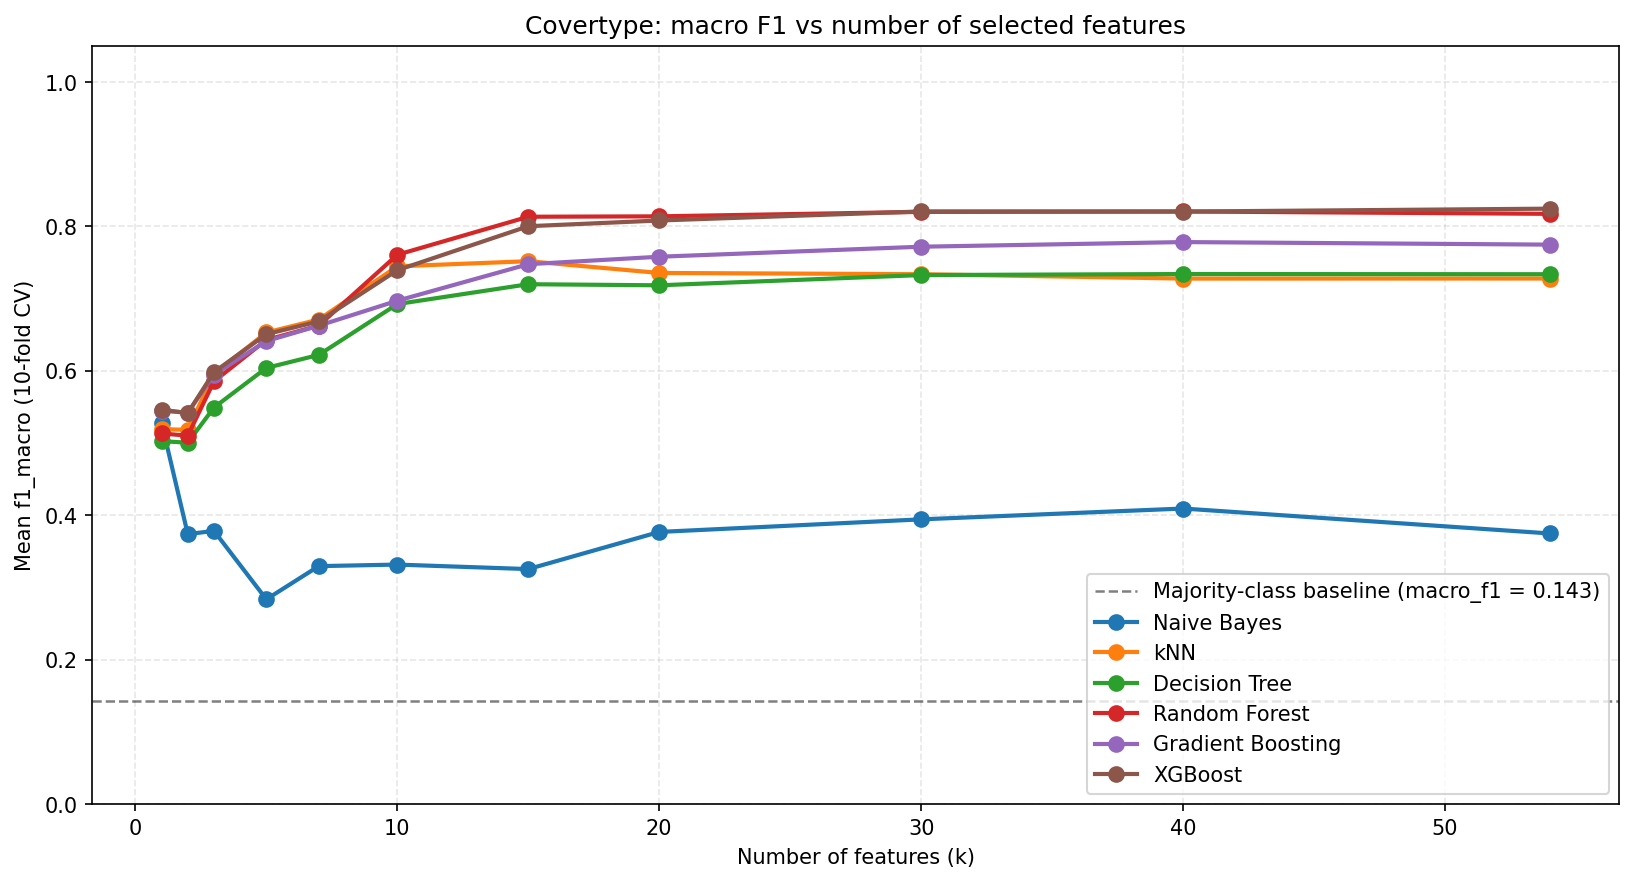
\includegraphics[width=0.95\textwidth]{feature_selection_sweep_f1_macro.png}
    \caption{Macro F1 versus number of selected features for all six
    classifiers on Covertype.}
    \label{fig:ct_fs_macro}
\end{figure}

Feature selection with $k = 30$ produces small or negligible effects for
every classifier. The largest positive effect --- for Naive Bayes --- is a
partial recovery from the scaling damage rather than a true improvement: the
absolute macro F1 of $0.394$ is still far below the raw-feature baseline of
$0.553$. For the tree-based ensembles, differences are within $\pm 0.004$ macro
F1 --- well within fold-to-fold noise.

The feature-selection sweep across $k \in \{1, \ldots, 54\}$
(Figure~\ref{fig:ct_fs_macro}) shows that all ensembles reach near-peak
performance by $k = 15$ and remain flat thereafter, indicating that fewer
than a third of the 54 available features carry the bulk of the
discriminative signal.

\paragraph{Which features drive the signal?}

To identify those features explicitly, the ANOVA F-statistic was computed
on the (scaled) training set for each of the 54 columns.
Table~\ref{tab:ct_top_features} lists the top 15 by F-score, together with
the family each feature belongs to. Two findings dominate the table.

First, \texttt{Elevation} alone has an F-statistic of $6113.8$, which is
$3.3\times$ the second-ranked feature (\texttt{Wilderness\_Area4},
$F = 1852.2$) and more than $12\times$ the third-ranked feature
(\texttt{Horizontal\_Distance\_To\_Roadways}, $F = 487.3$). No other column
comes close to Elevation's univariate discriminative power on this dataset.

Second, the top 15 features are split across all three feature families
present in the dataset: $5$ continuous cartographic measurements (including
all four distance-based measurements that rank in the top 15), $3$ of the
$4$ wilderness-area binary indicators, and $7$ of the $40$ soil-type binary
indicators. So the contention is not that ``useful features are concentrated
in the continuous columns'': both binary families contribute strongly. Each
family does, however, contribute at a different scale --- $5/10$ continuous
features land in the top 15 ($50\%$ of the family), against $3/4$ of the
wilderness areas ($75\%$) and only $7/40$ of the soil types ($17.5\%$).
The soil-type family is the most heterogeneous: a handful are highly
discriminative, but the majority rank in the bottom half by F-statistic.

The F-statistic falls off rapidly past the top 15: by rank 20 it is at
roughly $1\%$ of rank 1's value, and the remaining $\sim 35$ features
together account for very little incremental signal. This is exactly the
$k = 15$ saturation point visible in Figure~\ref{fig:ct_fs_macro}.

\begin{table}[H]
    \centering
    \caption{The 15 most discriminative individual features on the
    Covertype training set, ranked by the ANOVA F-statistic (computed on
    the scaled training data of the balanced subsample, 80/20 stratified
    split). Family membership uses the partitioning described in
    \S\ref{sec:covertype}.}
    \label{tab:ct_top_features}
    \begin{tabular}{rllr}
        \toprule
        Rank & Feature & Family & F-score \\
        \midrule
        1  & \texttt{Elevation}                          & Continuous cartographic & $6113.8$ \\
        2  & \texttt{Wilderness\_Area4}                  & Wilderness area         & $1852.2$ \\
        3  & \texttt{Horizontal\_Distance\_To\_Roadways} & Continuous cartographic & $487.3$  \\
        4  & \texttt{Soil\_Type3}                        & Soil type               & $371.0$  \\
        5  & \texttt{Soil\_Type10}                       & Soil type               & $349.7$  \\
        6  & \texttt{Wilderness\_Area1}                  & Wilderness area         & $324.1$  \\
        7  & \texttt{Soil\_Type38}                       & Soil type               & $301.9$  \\
        8  & \texttt{Horizontal\_Distance\_To\_Fire\_Points} & Continuous cartographic & $286.4$  \\
        9  & \texttt{Soil\_Type39}                       & Soil type               & $250.9$  \\
        10 & \texttt{Wilderness\_Area3}                  & Wilderness area         & $171.0$  \\
        11 & \texttt{Hillshade\_9am}                     & Continuous cartographic & $168.6$  \\
        12 & \texttt{Horizontal\_Distance\_To\_Hydrology} & Continuous cartographic & $146.6$  \\
        13 & \texttt{Soil\_Type30}                       & Soil type               & $142.0$  \\
        14 & \texttt{Soil\_Type40}                       & Soil type               & $139.9$  \\
        15 & \texttt{Soil\_Type29}                       & Soil type               & $122.2$  \\
        \bottomrule
    \end{tabular}
\end{table}

\paragraph{Principal Component Analysis.} PCA was not evaluated for
Covertype. As justified in Section~3.5.2, the dataset's mixed continuous
and one-hot encoded structure makes PCA components dominated by the variance
of the continuous columns; the resulting axes would not correspond to
interpretable cartographic categories.

% ---------------------------------------------------------------------
\subsubsection{Hyperparameter Sweep Analysis}\label{sec:ct_sweeps}
% ---------------------------------------------------------------------

For each tunable classifier (kNN, Decision Tree, Random Forest, Gradient
Boosting, and XGBoost) the two principal hyperparameters were swept using
10-fold stratified CV on the balanced training subsample, with the secondary
hyperparameter shown as separate lines on each plot and the remaining
hyperparameters held at their defaults. Each classifier was evaluated on
its Stage-2 best preprocessing configuration. Naive Bayes is omitted: the
variant used has no tunable hyperparameters in the search space considered.
All four scoring metrics --- accuracy, macro precision, macro recall, and
macro F1 --- are recorded for every cell.

\paragraph{k-Nearest Neighbors.}

Figure~\ref{fig:ct_sweep_knn} sweeps $k$ across 30 values from 1 to 150.
Every metric decreases monotonically with $k$ for all three distance
metrics, with Manhattan above Euclidean above Chebyshev throughout. The
best configuration sits at the smallest possible $k$: $k = 1$, Manhattan,
macro F1 $= 0.789$. The range across the sweep is unusually large for a
single classifier --- $0.488$ to $0.789$, a swing of $0.30$ macro F1. With
$\sim 5{,}600$ balanced training samples and seven well-separated cover
types, smoothing across neighbors pulls in samples from the wrong class
faster than it filters noise; the single nearest neighbor is the best
predictor available.

\begin{figure}[H]
    \centering
    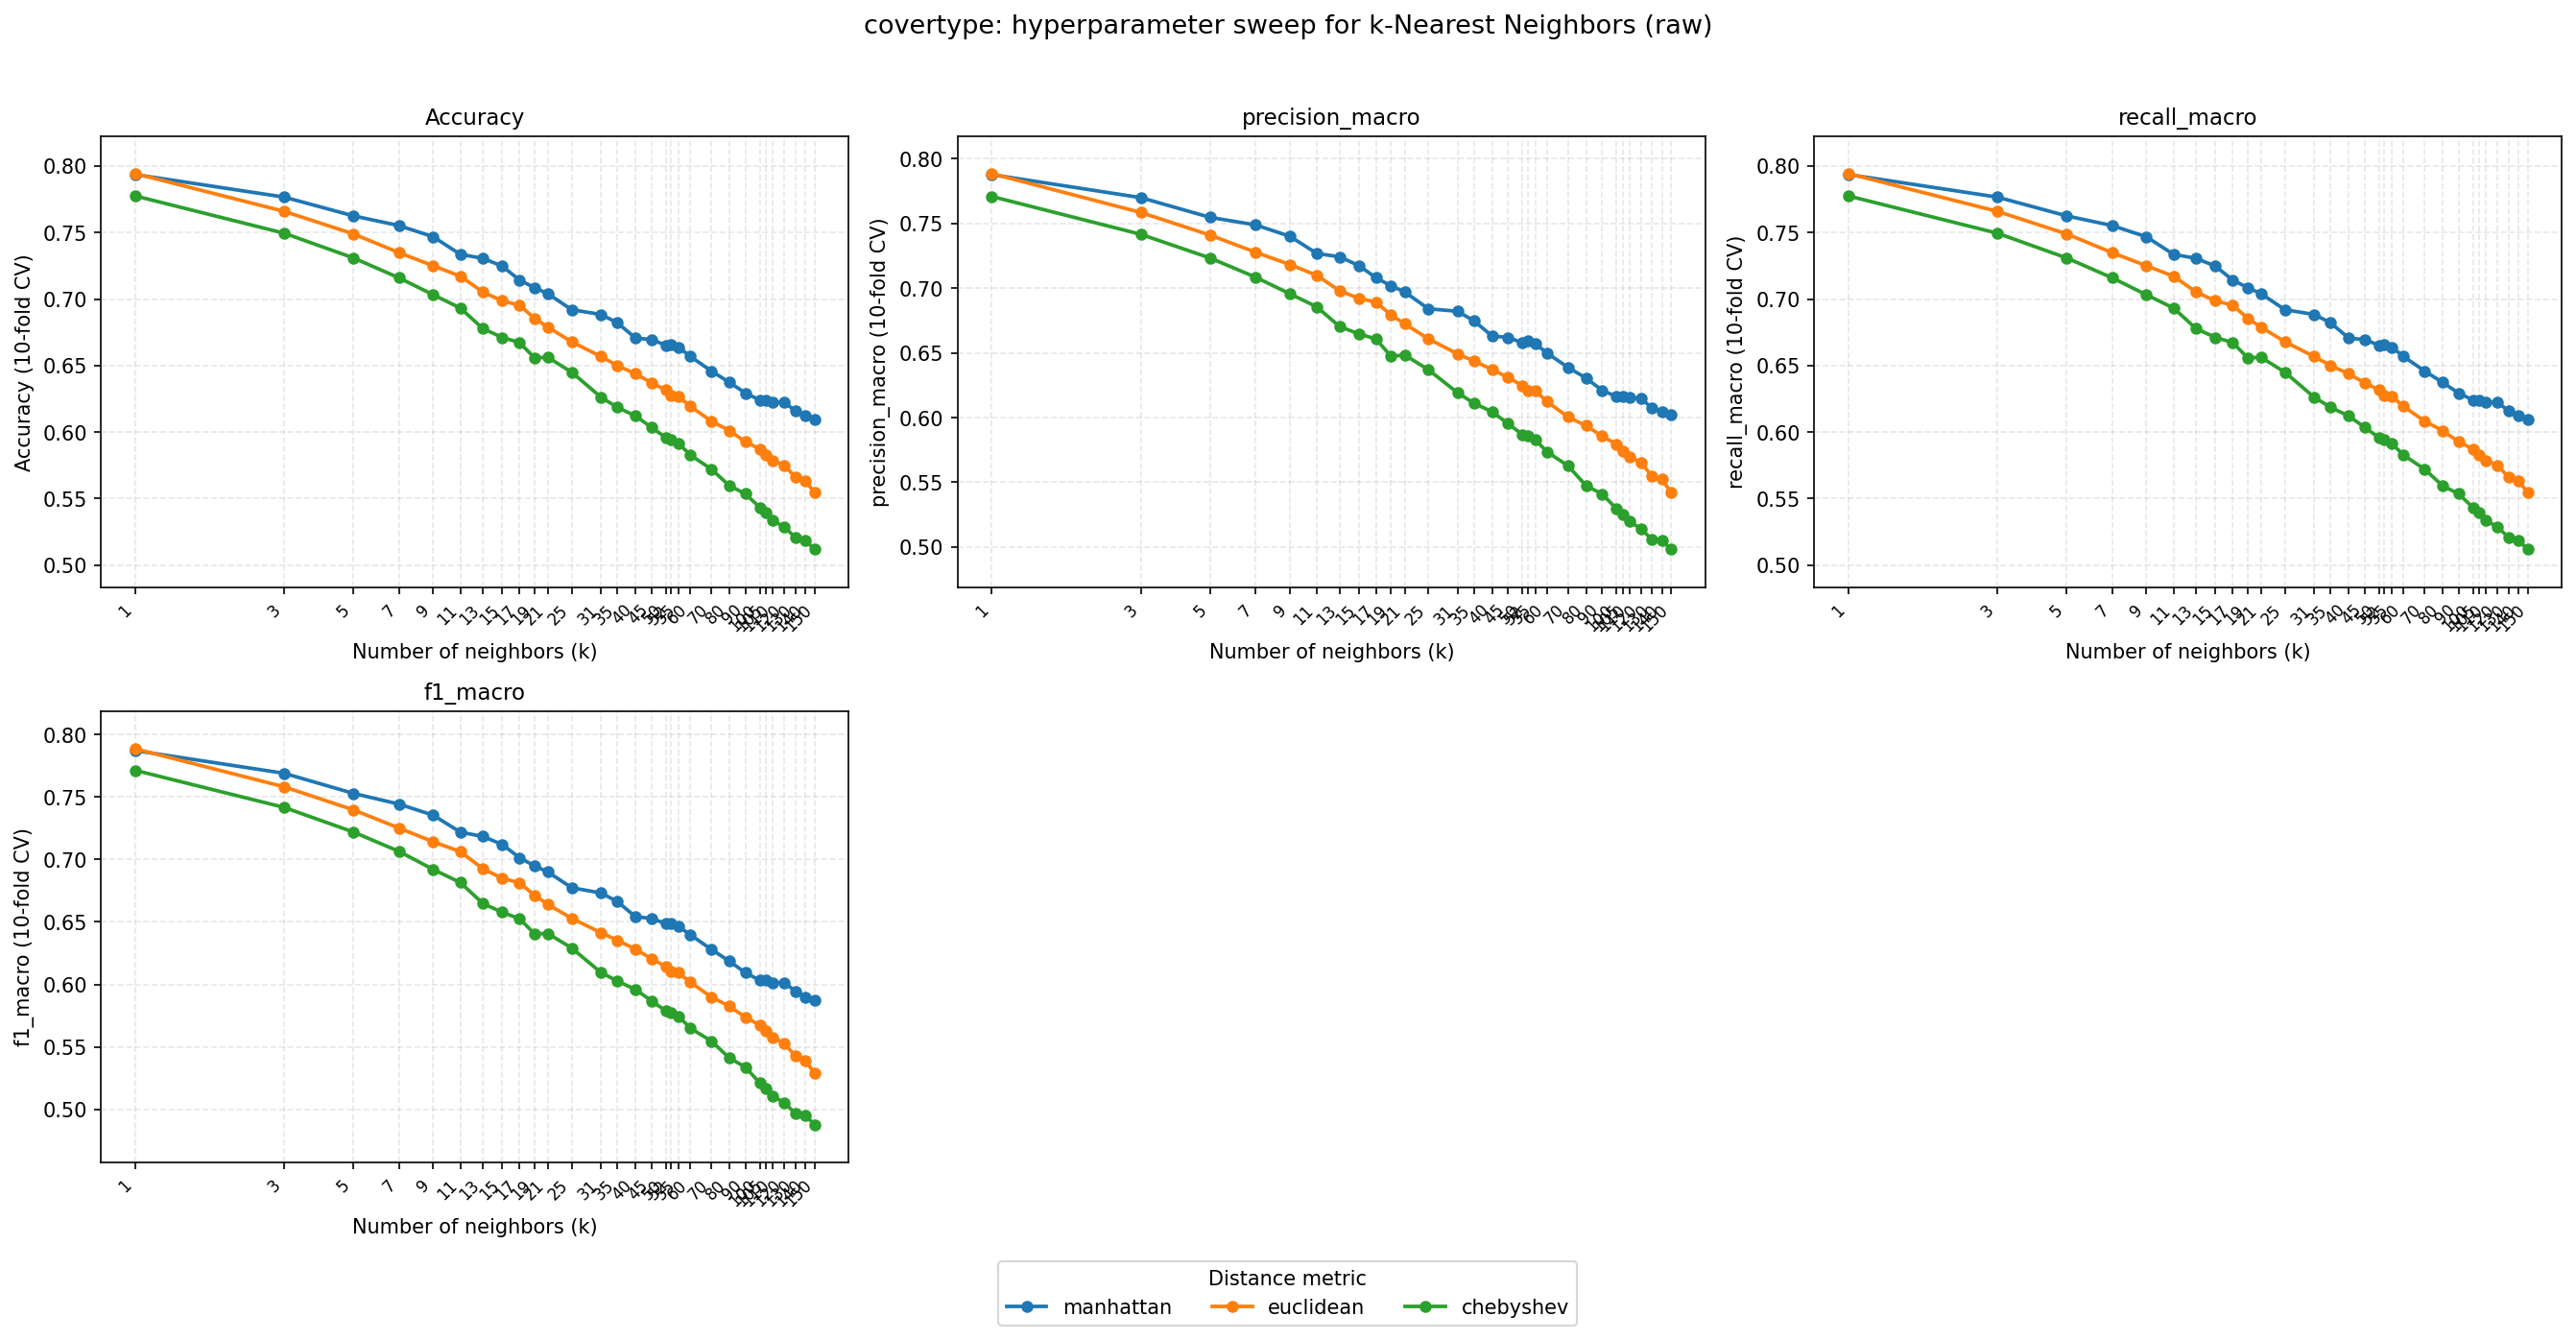
\includegraphics[width=\textwidth]{../artifacts/final/covertype/plots/classifier_sweep_knn.png}
    \caption{kNN hyperparameter sweep on Covertype: macro F1 and the three
    other scoring metrics versus the number of neighbors, segmented by
    distance metric.}
    \label{fig:ct_sweep_knn}
\end{figure}

\paragraph{Decision Tree.}

Figure~\ref{fig:ct_sweep_dt} shows the largest range of any classifier on
either dataset: macro F1 spans $0.344$ at \texttt{max\_depth} $= 2$ to
$0.719$ at \texttt{max\_depth} $= 10$. Three of the four
\texttt{min\_samples\_leaf} settings ($0.001$, $0.005$, $0.01$) converge
once depth exceeds $\sim 10$, while \texttt{min\_samples\_leaf} $= 0.05$
(requiring at least $\sim 280$ samples per leaf) plateaus much earlier and
much lower, around F1 $= 0.59$. The best configuration is \texttt{max\_depth}
$= 10$, \texttt{min\_samples\_leaf} $= 0.001$, F1 $= 0.719$. The contrast
with the corresponding Parkinson's sweep --- where \texttt{max\_depth} $= 2$
won --- comes from the sample-count asymmetry: deeper trees overfit Parkinson's
$\sim 200$ training samples but find more usable splits on Covertype's
$\sim 5{,}600$.

\begin{figure}[H]
    \centering
    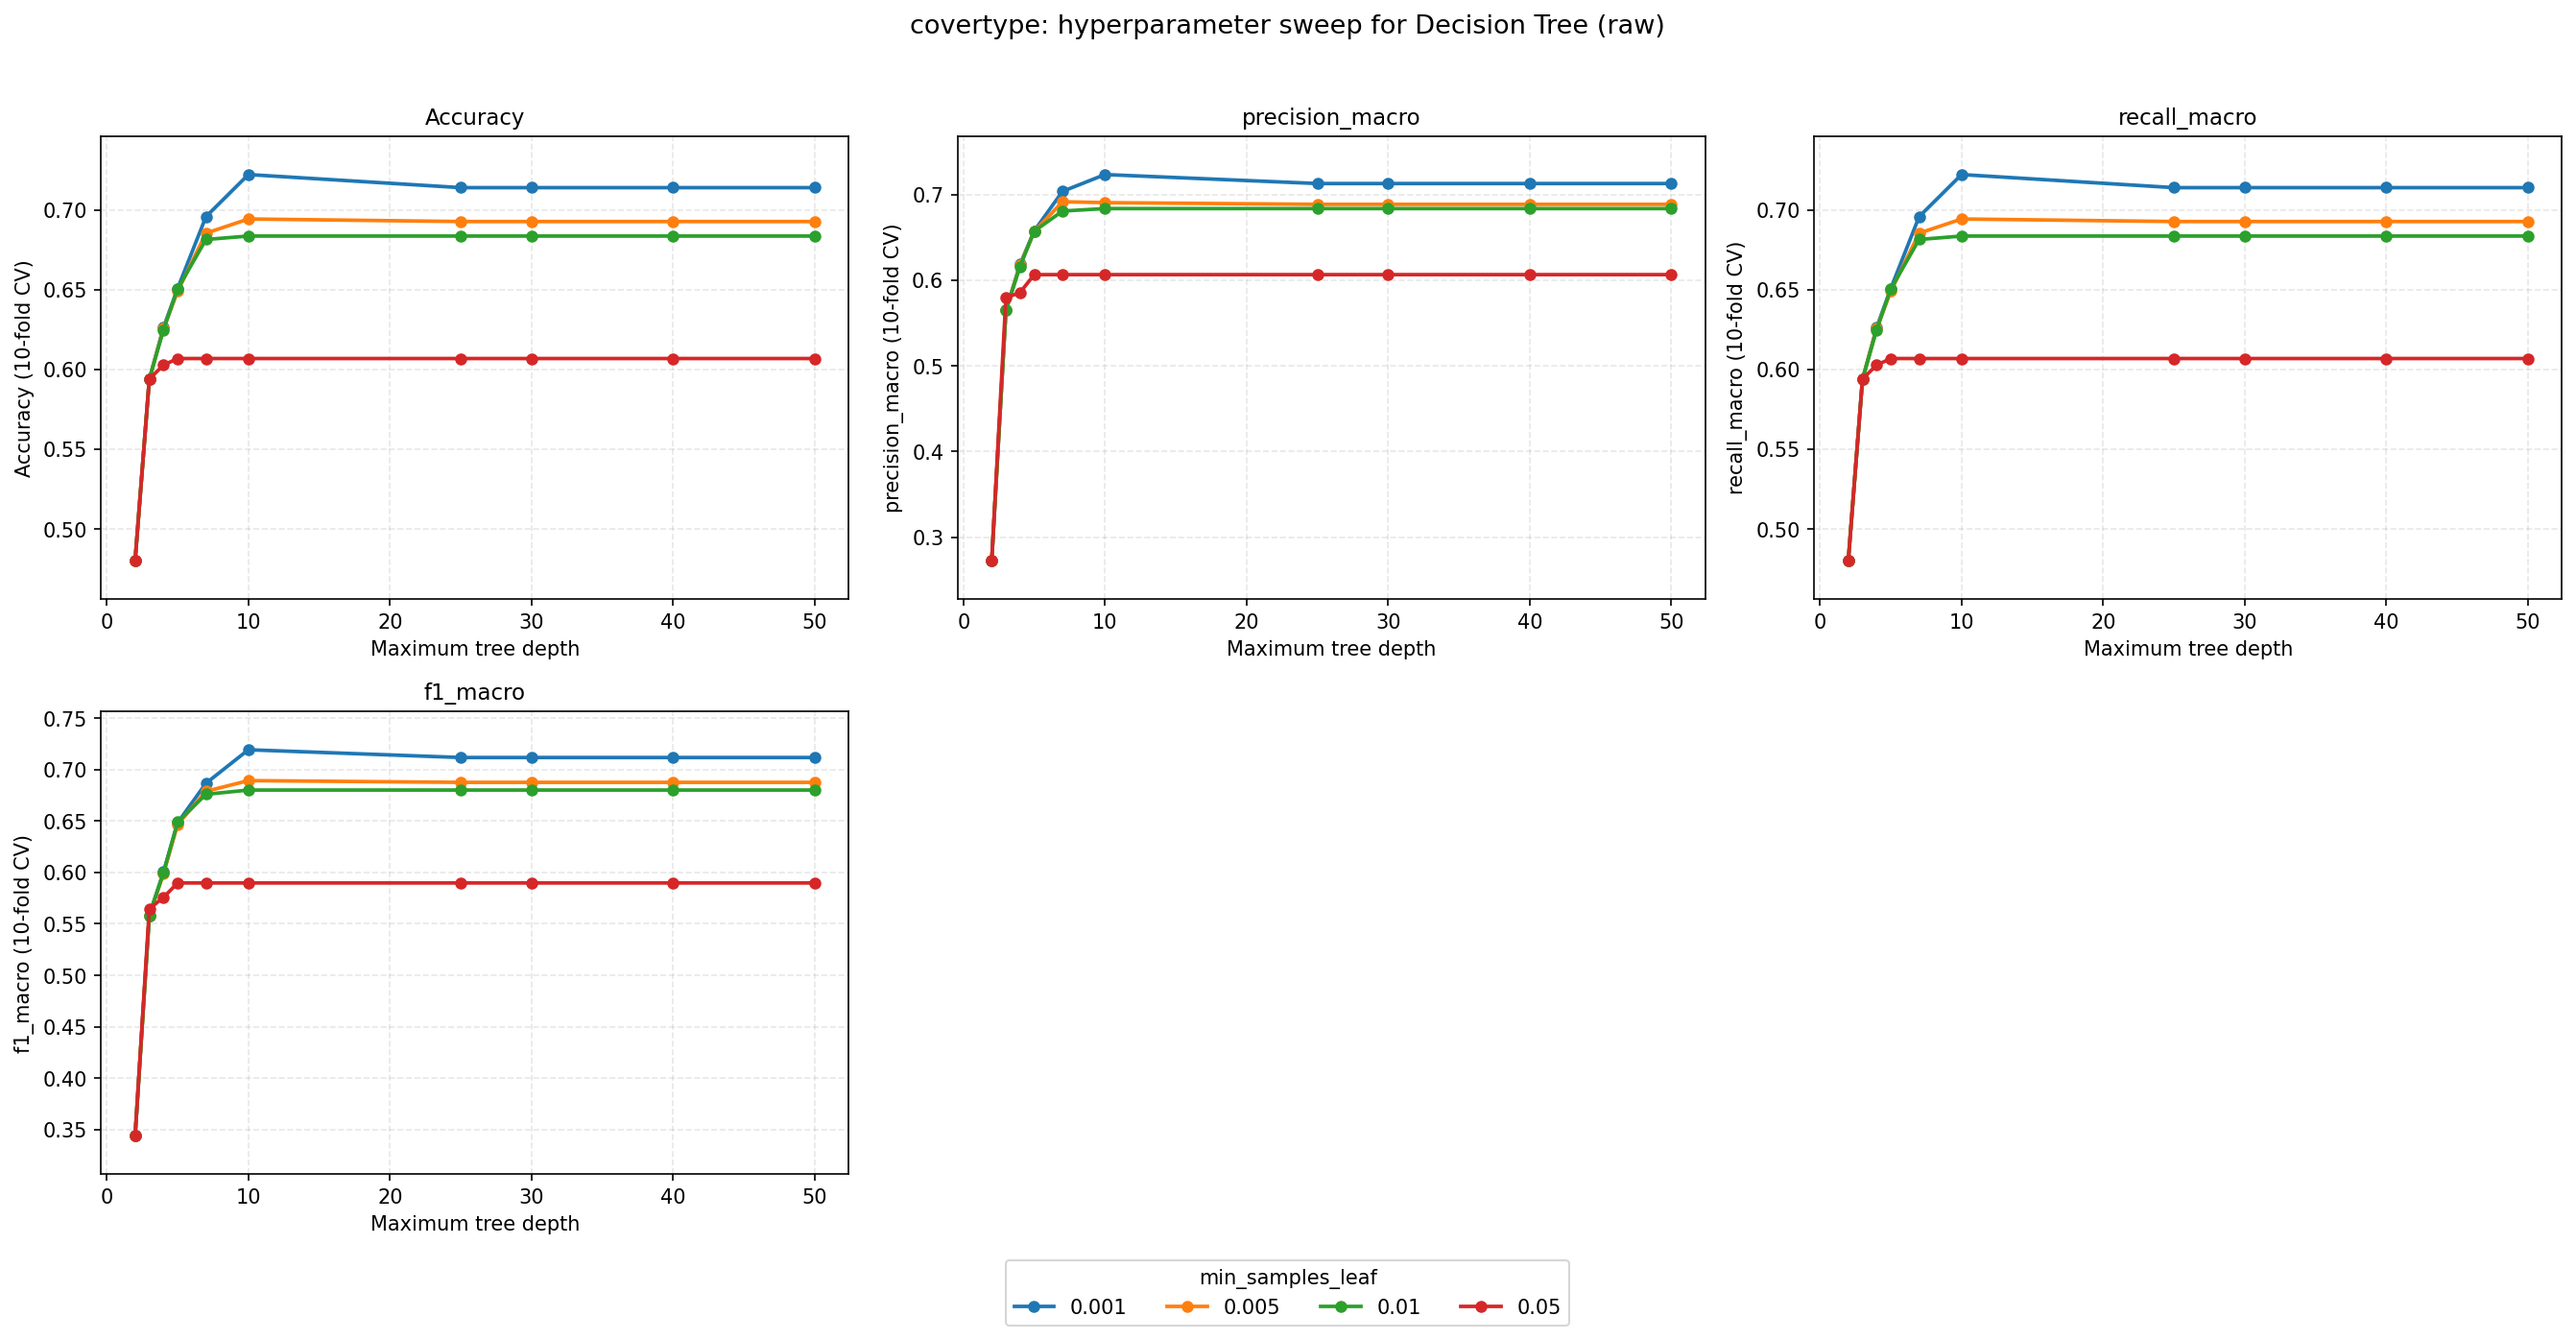
\includegraphics[width=\textwidth]{../artifacts/final/covertype/plots/classifier_sweep_decision_tree.png}
    \caption{Decision Tree hyperparameter sweep on Covertype: ten
    \texttt{max\_depth} values, four \texttt{min\_samples\_leaf} values.}
    \label{fig:ct_sweep_dt}
\end{figure}

\paragraph{Random Forest.}

Figure~\ref{fig:ct_sweep_rf} shows two distinct regimes. The
\texttt{max\_depth} $= 5$ line plateaus around macro F1 $= 0.70$ regardless
of \texttt{n\_estimators}, confirming that depth $5$ is too shallow to fit
the Covertype decision boundary. The \texttt{max\_depth} $= 25$ and
\texttt{max\_depth} $= 70$ lines, in contrast, are exactly coincident
across every \texttt{n\_estimators} value --- the same depth-saturation
effect as in the Parkinson's RF sweep, where individual trees stop
splitting because of pure leaves long before reaching the depth ceiling.
F1 rises from $\sim 0.76$ at $10$ trees to $\sim 0.82$ at $100$ and gains
little thereafter. Best configuration: $450$ trees, \texttt{max\_depth}
$= 70$, F1 $= 0.828$.

\begin{figure}[H]
    \centering
    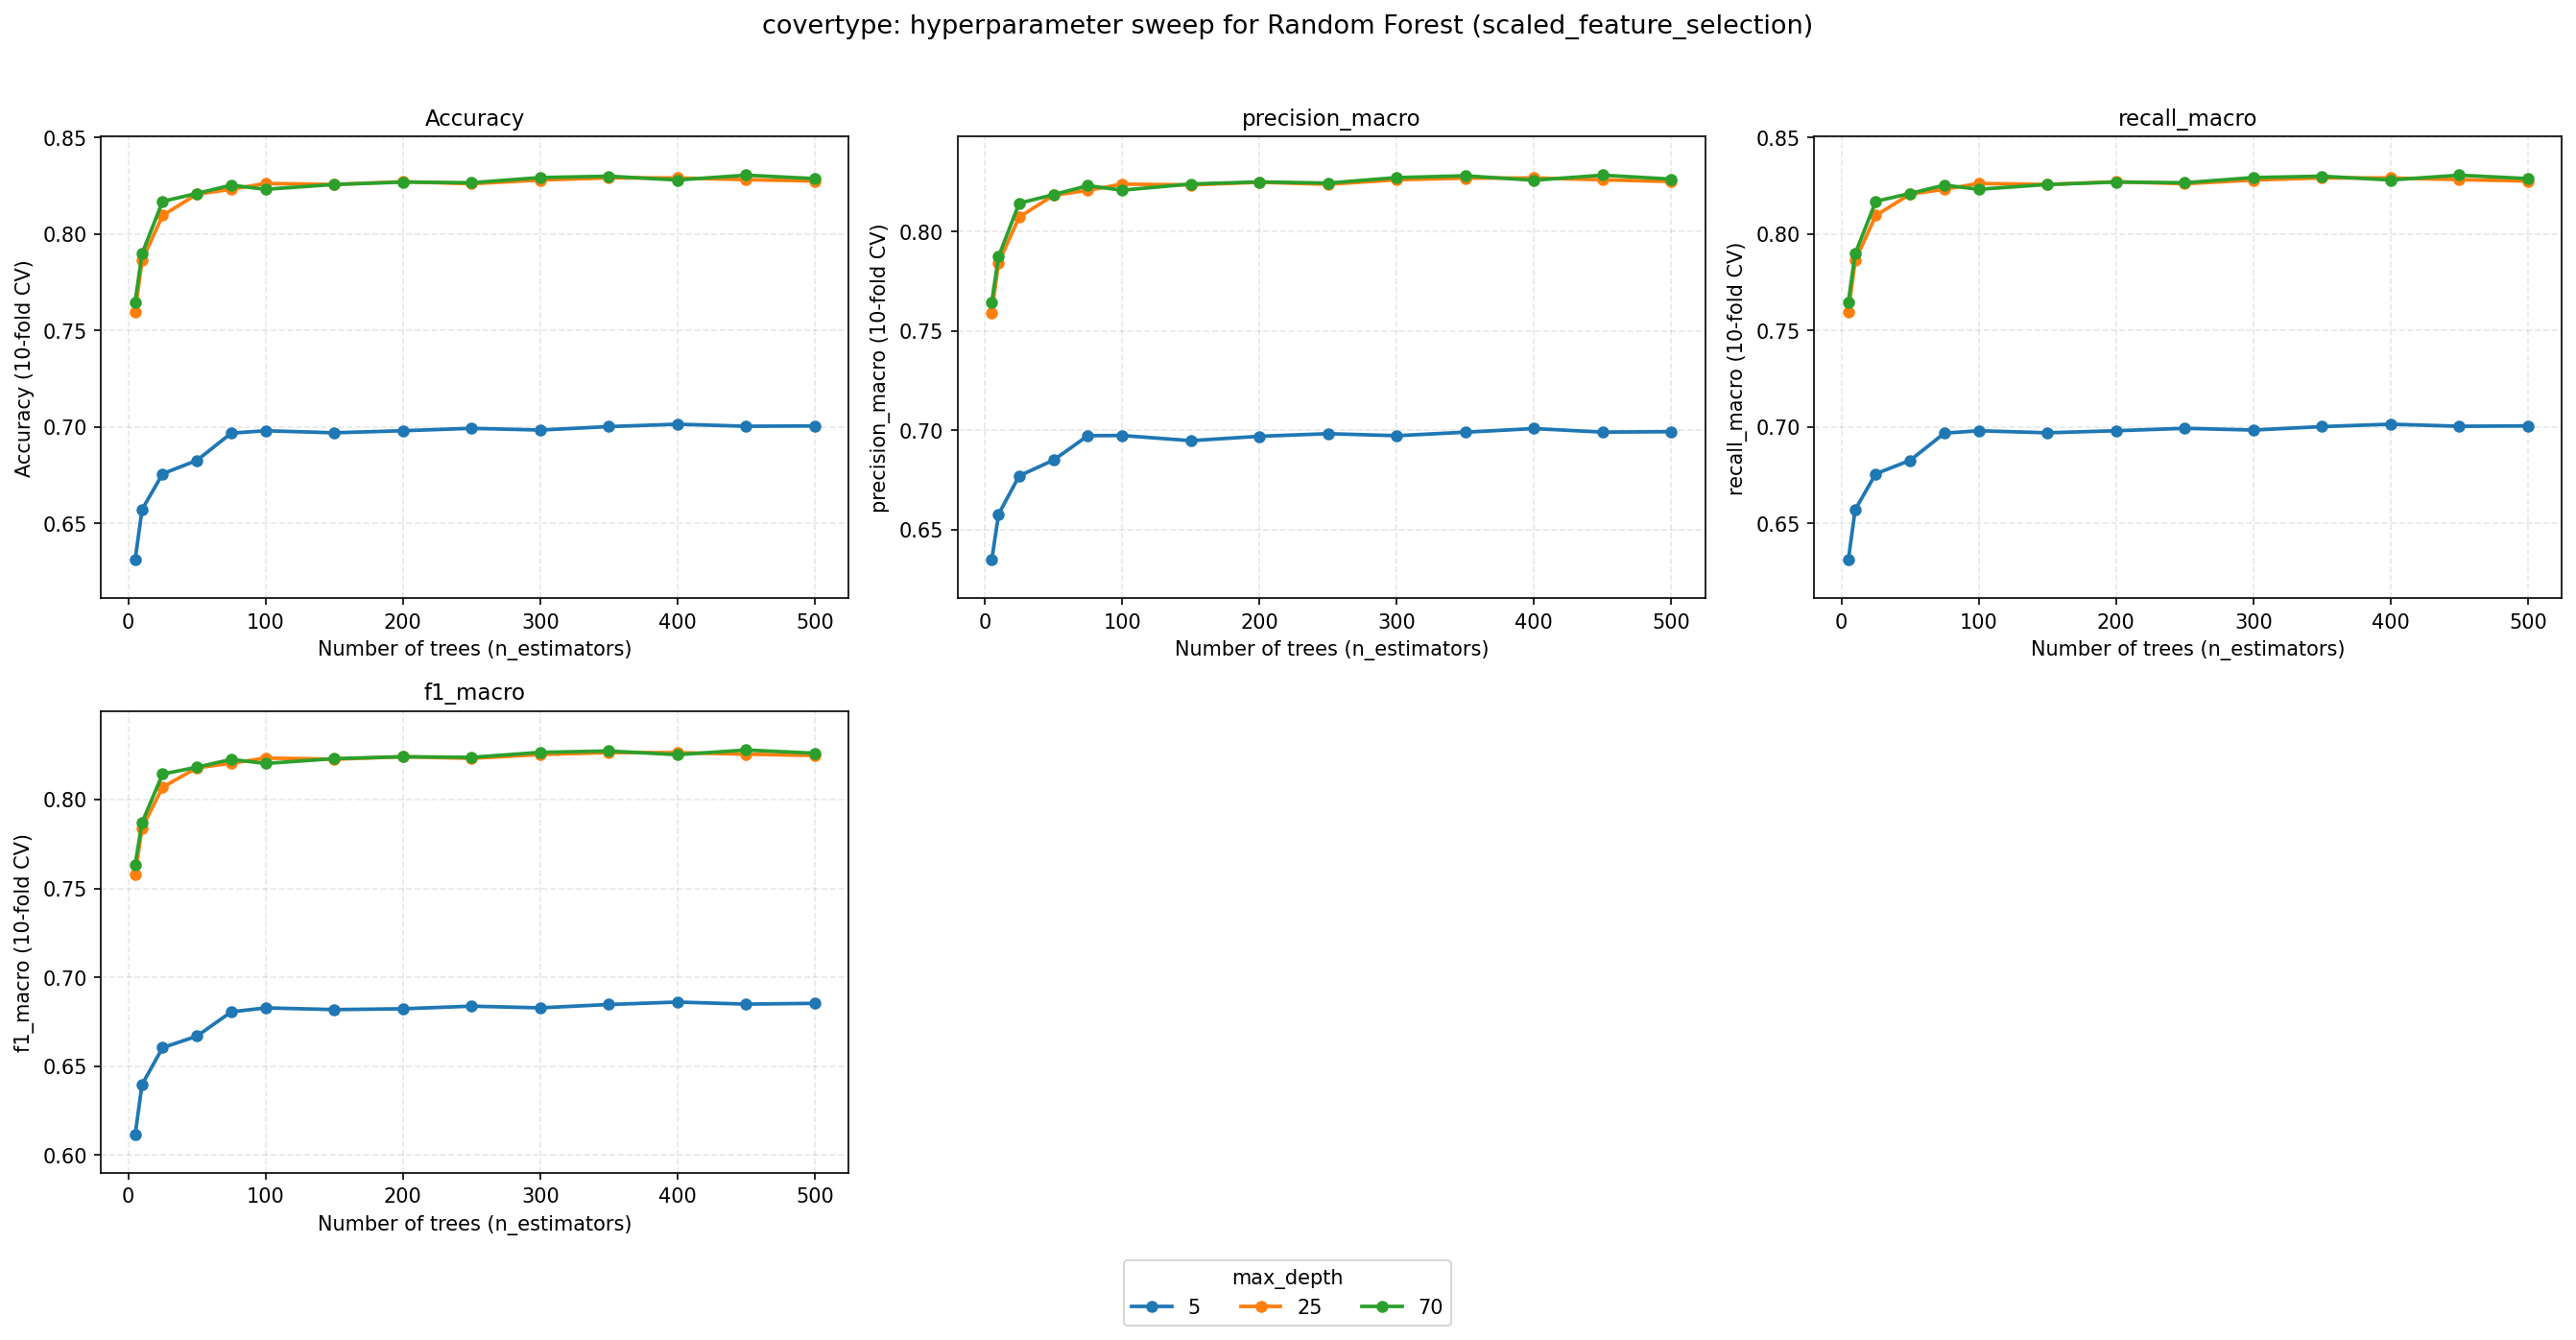
\includegraphics[width=\textwidth]{../artifacts/final/covertype/plots/classifier_sweep_random_forest.png}
    \caption{Random Forest hyperparameter sweep on Covertype: fourteen
    \texttt{n\_estimators} values, three \texttt{max\_depth} values.}
    \label{fig:ct_sweep_rf}
\end{figure}

\paragraph{Gradient Boosting.}

Figure~\ref{fig:ct_sweep_gb} shows that \texttt{max\_depth} $= 10$ dominates
both shallower (depth $5$) and deeper (depth $25$) alternatives across the
full range of \texttt{n\_estimators}. Macro F1 rises monotonically with
\texttt{n\_estimators} for depth $10$, reaching $0.832$ at $300$ estimators
and showing no plateau within the swept range --- a higher count might give
further (small) gains. Depth $25$ is competitive at low \texttt{n\_estimators}
but is overtaken by depth $10$ from about $100$ estimators onward and shows
clear signs of depth saturation past $n = 150$ (F1 frozen at $0.825$).
Gradient Boosting attains the highest macro F1 of any classifier on
Covertype, narrowly: $0.832$ versus XGBoost's $0.831$ and Random Forest's
$0.828$.

\begin{figure}[H]
    \centering
    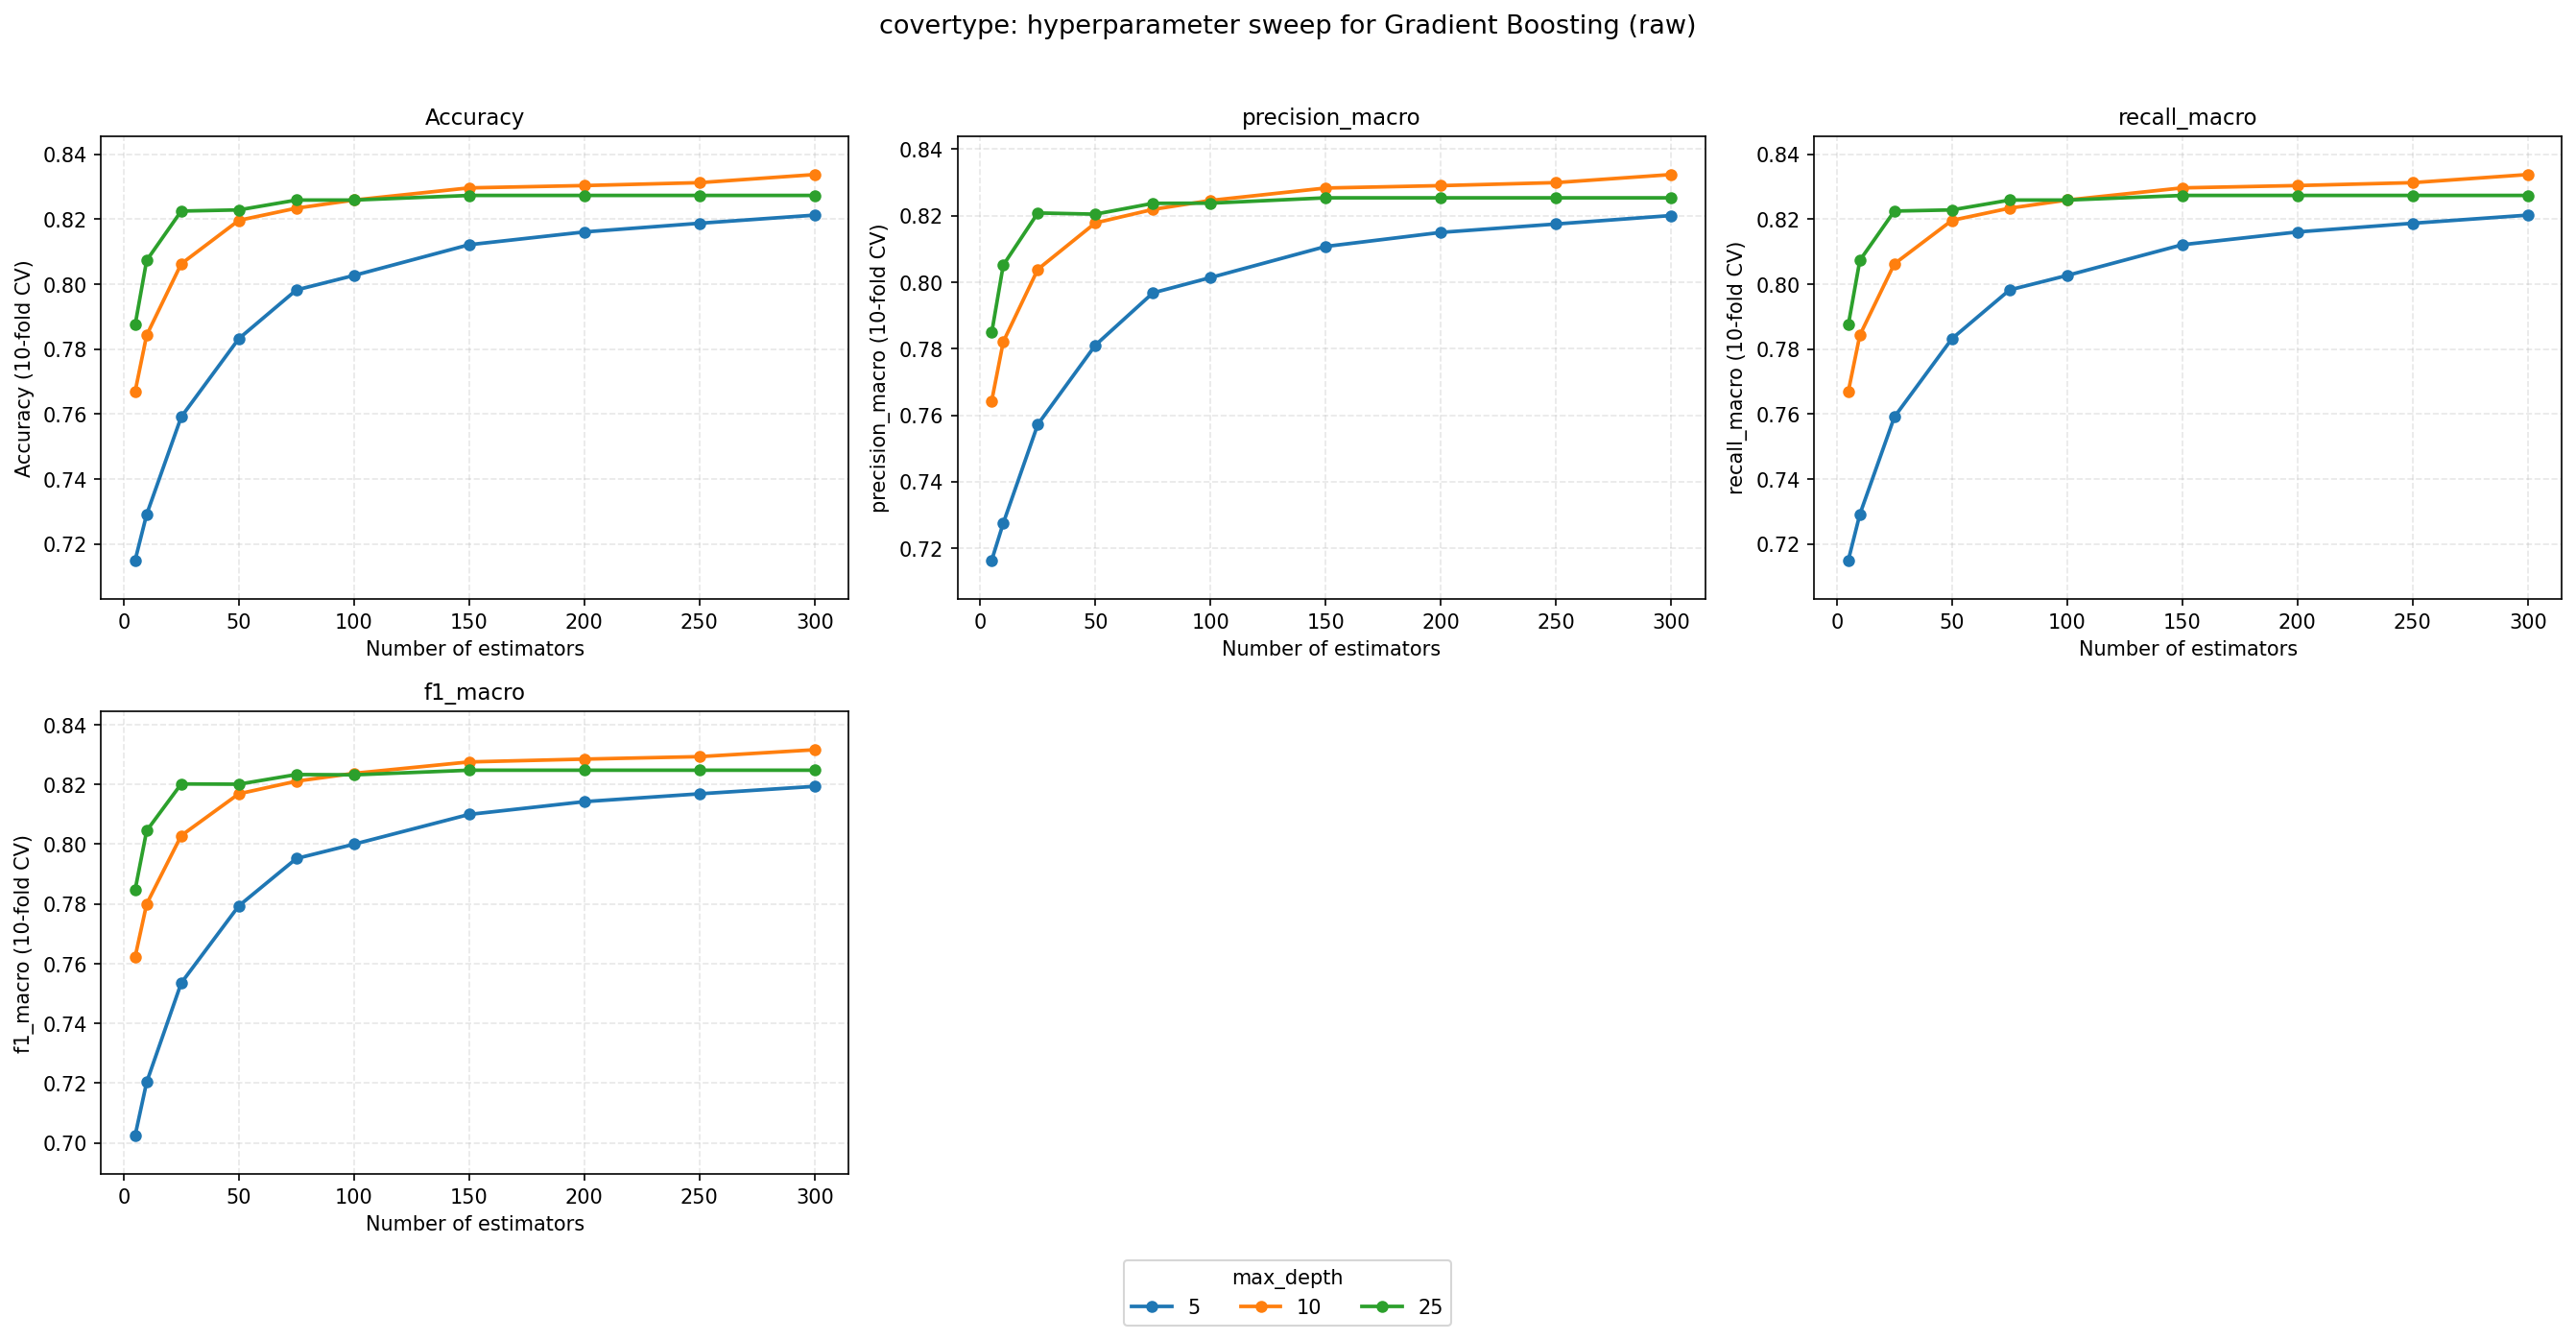
\includegraphics[width=\textwidth]{../artifacts/final/covertype/plots/classifier_sweep_gradient_boosting.png}
    \caption{Gradient Boosting hyperparameter sweep on Covertype: ten
    \texttt{n\_estimators} values, three \texttt{max\_depth} values.}
    \label{fig:ct_sweep_gb}
\end{figure}

\paragraph{XGBoost.}

Figure~\ref{fig:ct_sweep_xgb} shows the smallest variation of any classifier
on Covertype (macro F1 range $0.107$) but still reaches near the top of the
overall ranking. Depth $5$ under-fits and plateaus at F1 $\approx 0.81$;
depths $10$, $25$, and $50$ rise together rapidly and become essentially
indistinguishable past $n = 100$, with depths $25$ and $50$ exactly
coincident throughout (the same saturation effect as in Random Forest).
The best cell is \texttt{n\_estimators} $= 100$, \texttt{max\_depth} $= 25$,
F1 $= 0.831$ --- effectively tied with Gradient Boosting.

\begin{figure}[H]
    \centering
    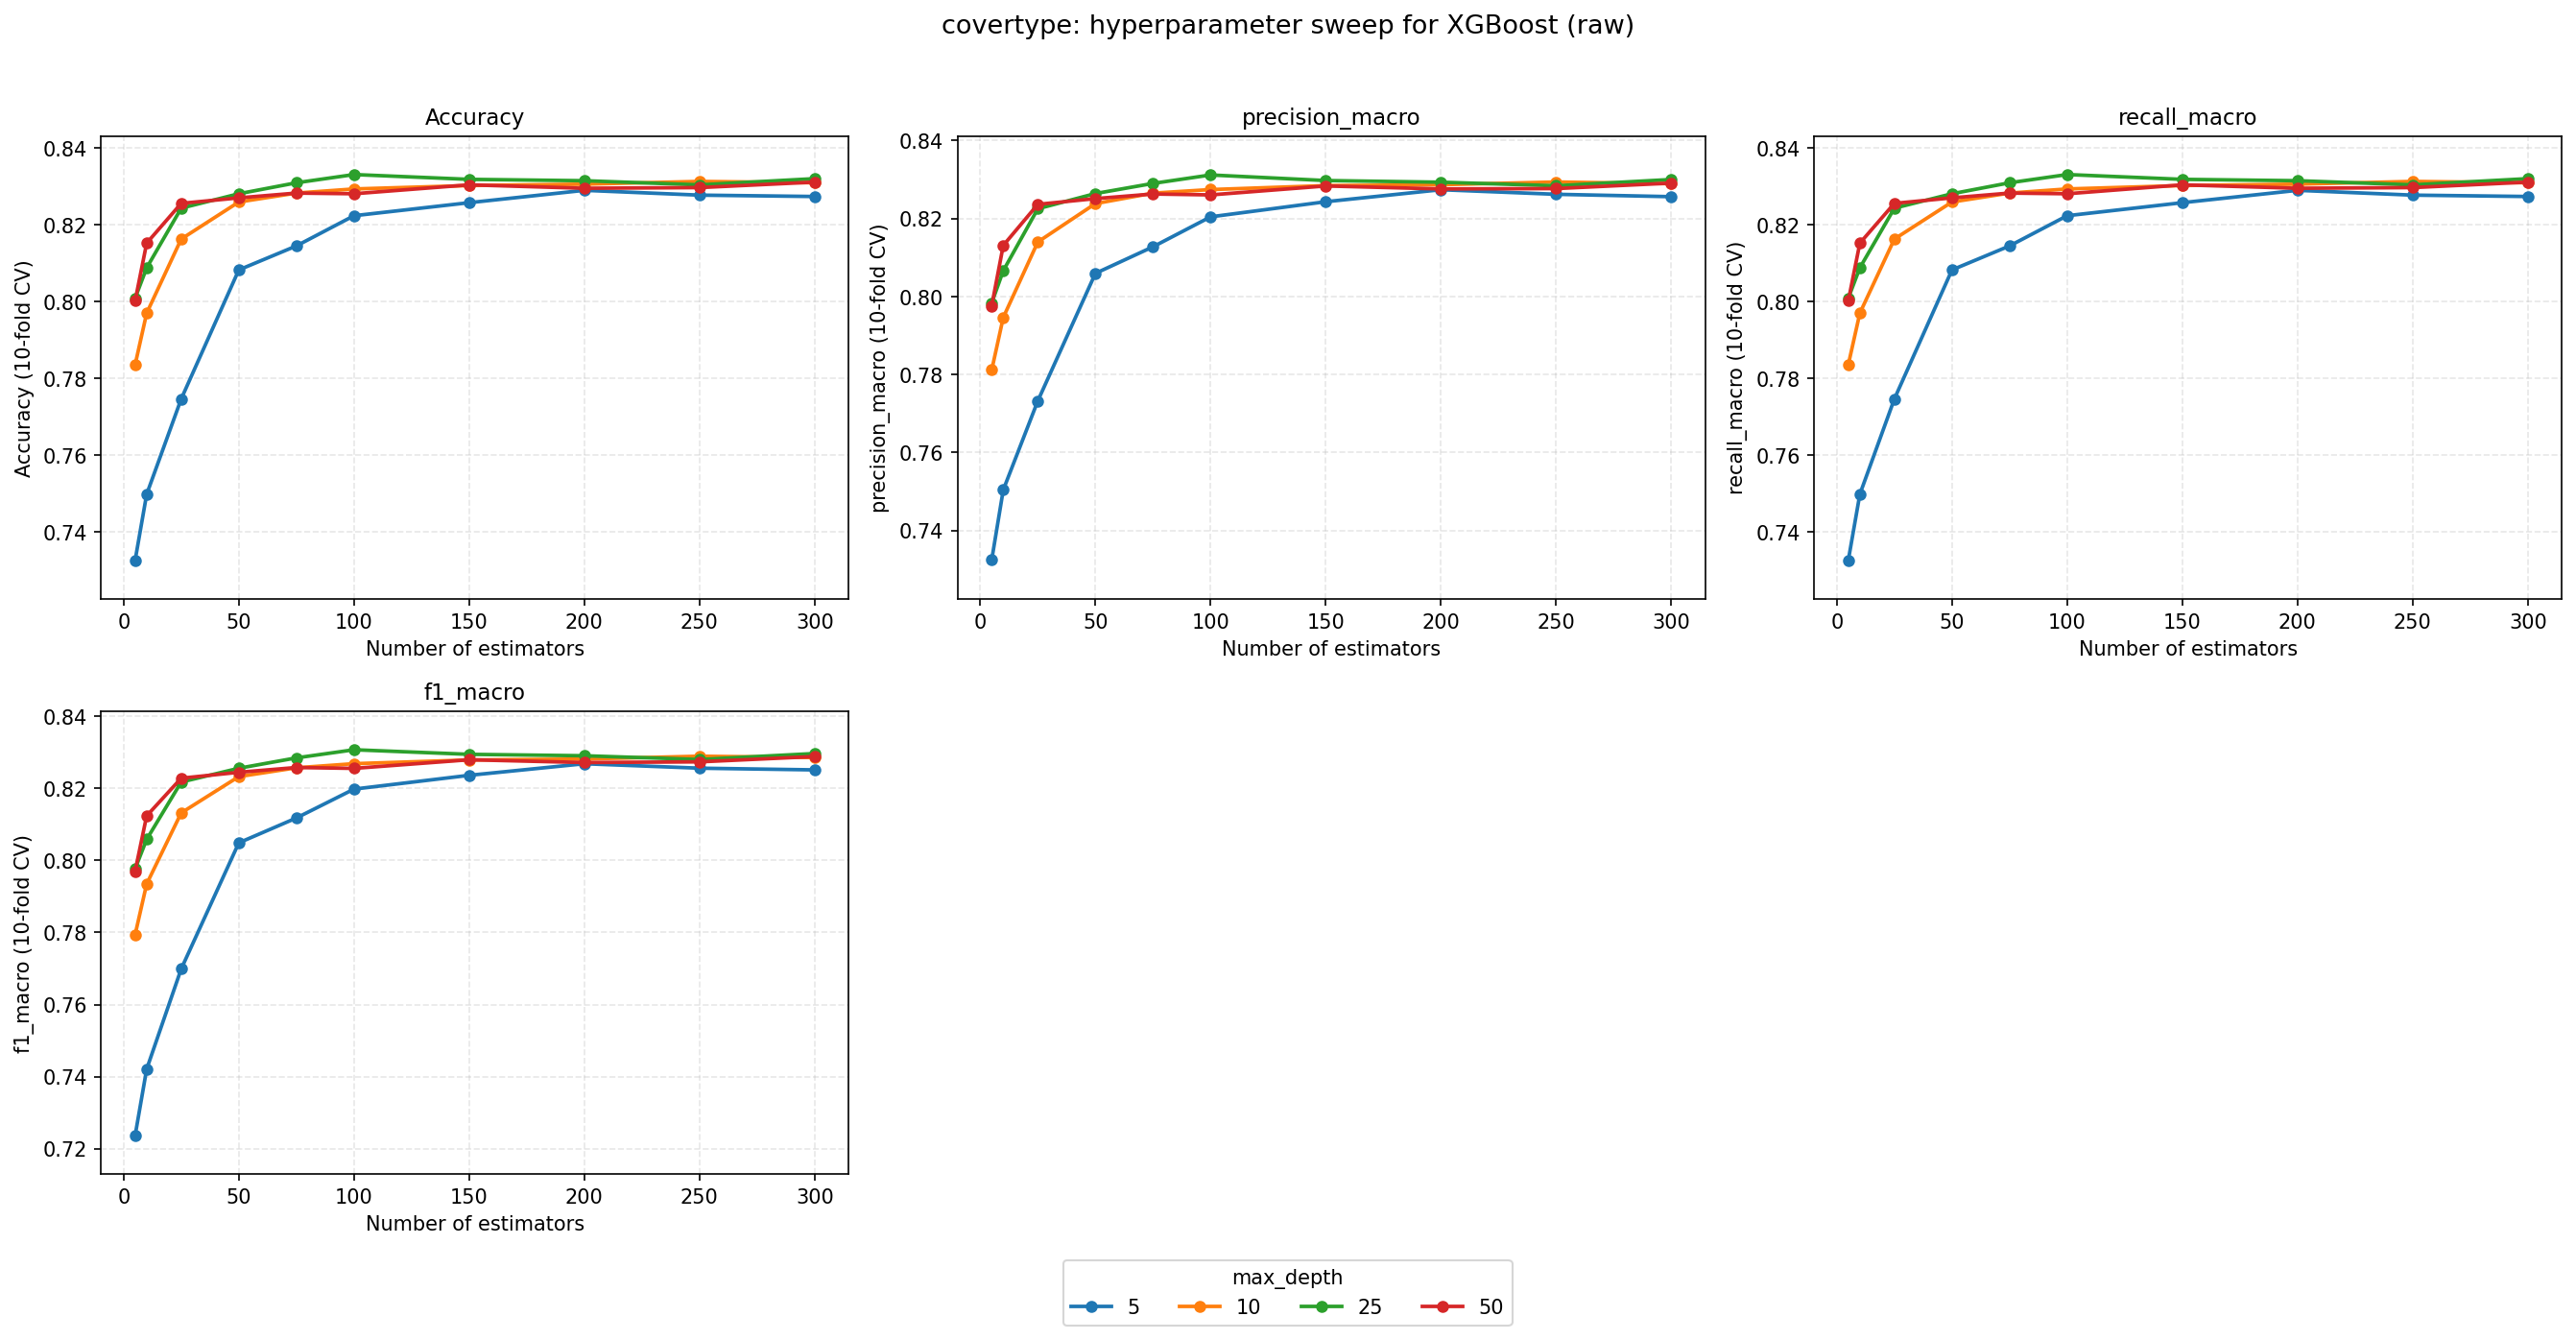
\includegraphics[width=\textwidth]{../artifacts/final/covertype/plots/classifier_sweep_xgboost.png}
    \caption{XGBoost hyperparameter sweep on Covertype: ten
    \texttt{n\_estimators} values, four \texttt{max\_depth} values.}
    \label{fig:ct_sweep_xgb}
\end{figure}

\paragraph{Cross-classifier synthesis.}

Ranking the five tunable classifiers by their best CV macro F1 across these
sweeps: Gradient Boosting ($0.832$), XGBoost ($0.831$), Random Forest
($0.828$), kNN ($0.789$), Decision Tree ($0.719$). The three tree-based
ensembles cluster within $0.005$ of each other --- essentially indistinguishable
on this dataset --- and beat the single Decision Tree by about $0.11$ F1, the
largest model-family gap of any sweep in this study. Two further
observations are worth flagging. First, hyperparameter sensitivity on
Covertype is far higher than on Parkinson's: even the most-stable classifier
(XGBoost) spans $0.107$ F1 across the swept grid, against Parkinson's
XGBoost which spanned only $0.018$. Most of this is driven by the under-fit
end of the curves --- shallow trees ($5$), tiny ensembles ($n \leq 10$), or
over-restrictive \texttt{min\_samples\_leaf} --- but the magnitude shows
that on a larger and more multi-class dataset, the choice of hyperparameter
is a much more consequential decision than the choice of preprocessing
configuration (cf.\ Table~\ref{tab:ct_overall}). Second, the same
depth-saturation pattern observed on Parkinson's --- where individual trees
stop splitting before reaching the depth ceiling --- recurs on Covertype's
Random Forest and XGBoost; this appears to be a property of the
\texttt{ColumnTransformer}-based training data rather than the algorithm,
and any \texttt{max\_depth} value above $\sim 25$ should be treated as
``no depth limit''.

% ---------------------------------------------------------------------
\subsubsection{Final Covertype Model and Per-Class Performance}\label{sec:ct_final}
% ---------------------------------------------------------------------

The best-performing model on Covertype was Gradient Boosting on raw
features, with tuned hyperparameters \texttt{learning\_rate}~$= 0.1$,
\texttt{max\_depth}~$= 10$, \texttt{n\_estimators}~$= 200$, and
\texttt{max\_features}~$= \sqrt{n}$. Refitting this configuration on the full
training set and evaluating on the held-out 20\% test split
($n = 1{,}400$, $200$ per class) produced the aggregate metrics in
Table~\ref{tab:ct_final}.

\begin{table}[H]
    \centering
    \caption{Test-set metrics for the tuned Gradient Boosting model on
    Covertype, broken down per class. The bottom block shows overall
    accuracy and the macro-averaged metrics. Classes are listed in their
    original label order (1--7).}
    \label{tab:ct_final}
    \begin{tabular}{lrrrr}
        \toprule
        Class & Precision & Recall & F1 & Support \\
        \midrule
        Spruce/Fir         & $0.768$ & $0.695$ & $0.730$ & $200$  \\
        Lodgepole Pine     & $0.680$ & $0.595$ & $0.635$ & $200$  \\
        Ponderosa Pine     & $0.857$ & $0.780$ & $0.817$ & $200$  \\
        Cottonwood/Willow  & $0.925$ & $0.985$ & $0.954$ & $200$  \\
        Aspen              & $0.786$ & $0.935$ & $0.854$ & $200$  \\
        Douglas-fir        & $0.826$ & $0.855$ & $0.840$ & $200$  \\
        Krummholz          & $0.926$ & $0.945$ & $0.936$ & $200$  \\
        \midrule
        Accuracy           &         &         & $0.827$ & $1{,}400$ \\
        Macro average      & $0.824$ & $0.827$ & $0.824$ & $1{,}400$ \\
        \bottomrule
    \end{tabular}
\end{table}

The macro F1 of $0.824$ is well above the seven-class balanced-class
random baseline of $1/7 \approx 0.143$ and tracks the cross-validation
estimate of $0.829$ from Table~\ref{tab:ct_overall} within $0.005$, a normal
held-out drop. Accuracy and macro recall coincide for the same reason noted in the
discussion below Table~\ref{tab:ct_overall}: every class has equal support
on the held-out split, so micro and macro recall coincide.

\begin{figure}[H]
    \centering
    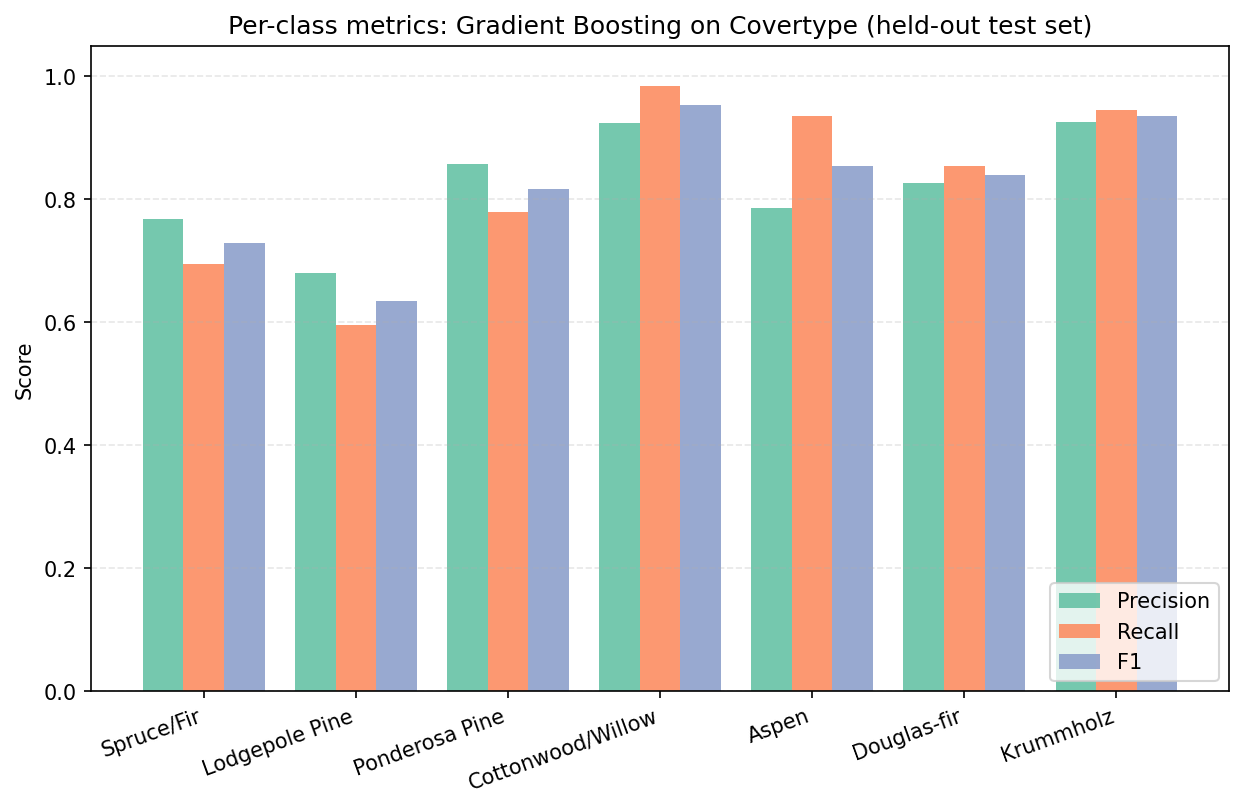
\includegraphics[width=0.85\textwidth]{best_model_per_class.png}
    \caption{Per-class precision, recall, and F1-score for the best Covertype
    model on the held-out test set. Cottonwood/Willow and Krummholz achieve
    F1 above 0.94, while Lodgepole Pine plateaus around 0.63 due to
    systematic confusion with Spruce/Fir.}
    \label{fig:ct_per_class_bars}
\end{figure}

\begin{figure}[H]
    \centering
    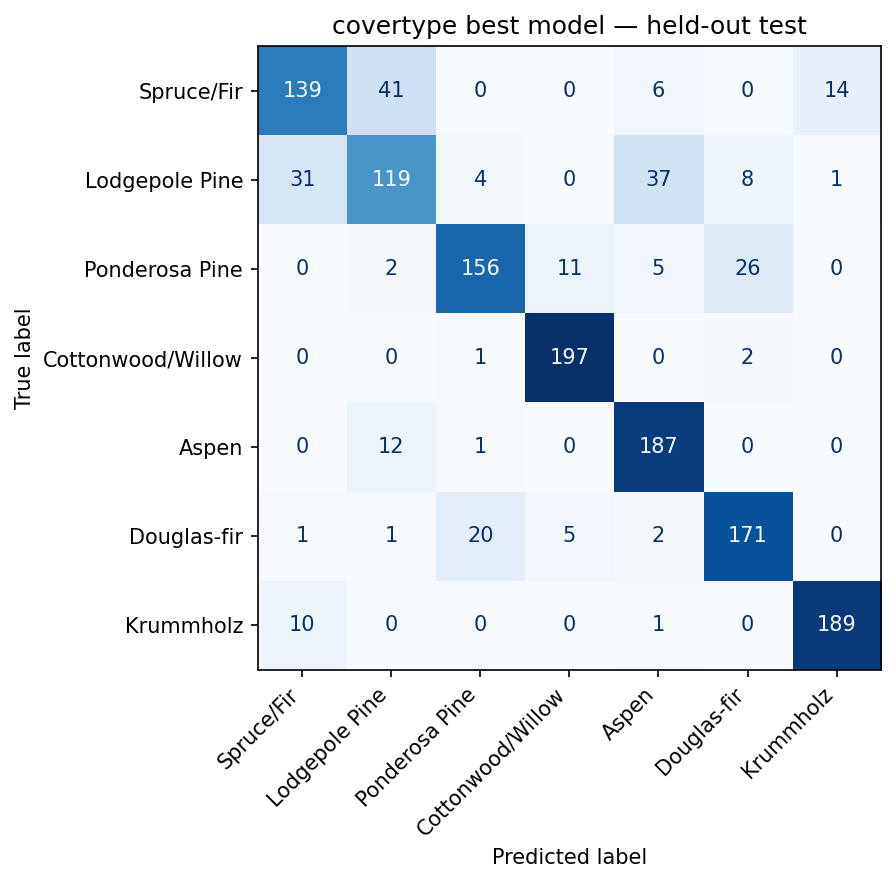
\includegraphics[width=0.8\textwidth]{../artifacts/final/covertype/confusion_matrix.png}
    \caption{Confusion matrix for the best Covertype model on the held-out
    test set. The systematic confusion between Spruce/Fir and Lodgepole Pine
    is visible as the off-diagonal entries in the top-left of the matrix.}
    \label{fig:ct_confusion}
\end{figure}

The per-class results in Figure~\ref{fig:ct_per_class_bars} reveal three
distinct behavioural tiers among the seven cover types:

\begin{itemize}
    \item \textbf{Cottonwood/Willow} (F1 0.95) and \textbf{Krummholz}
    (F1 0.94) classify cleanly. Cottonwood/Willow grows near streams,
    captured by the distance-to-hydrology feature; Krummholz is the
    high-elevation tree-line species, captured by elevation alone.
    \item \textbf{Aspen, Douglas-fir, Ponderosa Pine, Spruce/Fir} occupy a
    middle band with F1 between 0.73 and 0.85.
    \item \textbf{Lodgepole Pine} (F1 0.63) is the worst-performing class.
    This is the dominant source of error in the confusion matrix: 41 actual
    Spruce/Fir samples are misclassified as Lodgepole Pine, and 31 actual
    Lodgepole Pine samples are misclassified as Spruce/Fir. The two species
    coexist at similar elevations with overlapping cartographic profiles, so
    the available features do not separate them cleanly.
\end{itemize}

The macro F1 ceiling of 0.82 is bounded not by classifier capacity but by
intrinsic feature limitations: no amount of feature engineering can separate
Lodgepole Pine from Spruce/Fir using the cartographic variables available.
Improving this would require new features (e.g., tree morphology, soil
moisture, climate normals) rather than further model tuning.

% =====================================================================
\subsection{Comparison Between Datasets}\label{sec:comparison}
% =====================================================================

Gradient Boosting wins on both datasets: F1 $= 0.900$ on Parkinson's
(Table~\ref{tab:pd_overall}) and macro F1 $= 0.829$ on Covertype
(Table~\ref{tab:ct_overall}). On both, the tree-based ensembles --- Random
Forest, Gradient Boosting, XGBoost --- cluster tightly at the top
($\leq 0.005$ apart within each dataset). The gap between the ensembles and
the simpler classifiers (Decision Tree, Naive Bayes), however, is much wider
on Covertype than on Parkinson's: Covertype's $\sim 5{,}600$ training
samples give the ensembles more room to exploit the bias--variance trade-off
than Parkinson's $\sim 200$ do.

Preprocessing has a measurably larger effect on Parkinson's, while
hyperparameter choice has a much larger effect on Covertype. The largest
single preprocessing effect in either dataset is the $+0.06$ F1 gain that
scaling produces for kNN on Parkinson's (against essentially zero on
Covertype); the largest single hyperparameter sweep range is the $0.37$
Decision Tree macro F1 spread on Covertype (against $0.05$ on Parkinson's).
The same intervention can also flip in optimal value: Decision Tree's best
\texttt{max\_depth} is $2$ on Parkinson's (where deeper trees overfit) and
$10$ on Covertype (where shallower trees underfit), and kNN's best $k$ is
$35\text{--}50$ on Parkinson's (smoothing across neighbours helps) and $1$
on Covertype (smoothing pulls in samples from the wrong class). Sample
count is the unifying explanation.

The two datasets impose qualitatively different evaluation challenges.
Parkinson's $75/25$ class imbalance biases every classifier toward
predicting PD: recall sits above $0.95$ for the top four classifiers, while
Healthy-class specificity is much lower (the chosen model reaches PD recall
$0.99$ but Healthy recall only $0.48$). Covertype's seven balanced classes
avoid this aggregate asymmetry but reveal a feature-limited per-class
ceiling: Lodgepole Pine and Spruce/Fir share enough of their cartographic
profile that the final model confuses them systematically
(Figure~\ref{fig:ct_confusion}), capping macro F1 around $0.82$ regardless
of hyperparameter choice. On Parkinson's, the next lever would be threshold
tuning or class weighting; on Covertype, additional features.

% =====================================================================
\section{Conclusion}\label{sec:conclusion}
% =====================================================================

\subsection{Summary of Main Findings}

This study compared preprocessing strategies and classification algorithms
on two different classification problems: Parkinson's disease prediction
from speech recordings and forest cover type prediction from cartographic
variables. The results showed that model performance depends strongly on
both the dataset characteristics and the classifier family. Tree-based
ensemble methods, especially Gradient Boosting, Random Forest, and XGBoost,
were the most consistent performers across both datasets.

\subsection{Parkinson's Disease Findings}

For the Parkinson's disease dataset, Gradient Boosting achieved the
strongest tuned performance and was selected as the final model. The
model achieved high overall performance and very high recall for
Parkinson's disease cases, meaning that it correctly identified most PD
recordings. However, the per-class analysis showed that healthy controls
were much harder to classify. The model tended to favour the PD class,
which is consistent with the moderate class imbalance in the dataset.

The preprocessing analysis showed that scaling was especially important
for k-Nearest Neighbors, while tree-based models were mostly unaffected by
scaling. Feature selection and PCA confirmed that the Parkinson's feature
space contains substantial redundancy, since competitive performance could
be maintained after reducing the number of features. However, these
dimensionality-reduction methods did not fully solve the weaker
healthy-control detection.

\subsection{Covertype Findings}

For the Covertype dataset, Gradient Boosting, XGBoost, and Random Forest
achieved the strongest results on the balanced 7,000-record subset. The
final model clearly outperformed the majority-class baseline and achieved
strong macro-level performance. Scaling had little benefit for most models
and even harmed some classifiers, showing that preprocessing effects do
not transfer uniformly across datasets.

The per-class results showed that some cover types were easier to classify
than others. Cottonwood/Willow and Krummholz achieved the strongest
class-level performance, while Lodgepole Pine and Spruce/Fir were more
frequently confused. This suggests that the available cartographic features
do not separate all forest classes equally well.

\subsection{Limitations}

The main limitation of the Parkinson's experiment is that the final model
achieved much stronger performance on the PD class than on the
healthy-control class. Therefore, high overall F1-score should not be
interpreted as balanced performance across both classes. For the Covertype
dataset, the main limitation is that the experiments were conducted on a
balanced undersampled subset rather than the original imbalanced dataset.
As a result, the reported Covertype performance reflects the controlled
balanced setting, not necessarily performance on the natural class
distribution.

\subsection{Future Work}

Future work on the Parkinson's dataset should investigate imbalance-aware
strategies such as threshold tuning or class weighting. These approaches
may improve healthy-control recall while preserving strong PD detection.
For the Covertype dataset, future work should evaluate the selected models
on the original imbalanced distribution and investigate whether additional
geographic or ecological variables could reduce confusion between similar
classes such as Lodgepole Pine and Spruce/Fir.

\end{document}
